% \documentclass[aps,prb,superscriptaddress,showpacs,amsmath,amssymb,letterpaper]{revtex4}
% \usepackage{graphicx}
% \usepackage{epsfig,color,verbatim} % multi-line comments
% \usepackage{subfigure}             % allows for use of "sub figure" 1a, 1b, etc
% \usepackage{hyperref}

%\begin{document}

\chapter{Lorem ipsum dolor sit amet, consectetur adipiscing elit; Maecenas ultrices egestas commodo}
\label{chap:TE_gain}
\label{paper:1_start}

% \author{Ben Payne$^{1}$, Jonathan Andreasen$^{2}$, Hui Cao$^{2}$, and Alexey Yamilov$^{1}$\footnote{Email: yamilov@mst.edu}\\
\begin{center}
Ben Payne$^1$, Jonathan Andreasen$^2$, Hui Cao$^2$, and Alexey Yamilov$^1$      \label{sec:TE2009}                                                                         \end{center}

\ \\
\begin{center}
\textit{$^1$Department of Physics, Missouri University of Science \& Technology,\\ Rolla, MO 65409\\
$^2$Department of Applied Physics, Yale University, New Haven, CT 06520}\end{center}

\ \\
% {\it $^{1}$Department of Physics, Missouri University of Science \& Technology, Rolla, MO 65409\\
% $^{2}$Department of Applied Physics, Yale University, New Haven, CT 06520}}
% \noaffiliation
% \date{\today}
% \begin{abstract}
\addcontentsline{toc}{section}{ABSTRACT}
\begin{center}\textbf{ABSTRACT\footnote{Published in Physical Review B \textbf{82} 104204 (2010).}}        \end{center}

In this work, we investigate a possibility of using the ratio between optical transmission, $T$, and energy stored inside the system, ${\cal E}$, as a quantitative measure of the enhanced mesoscopic corrections to diffusive transport of light through a random medium with gain. We obtain an expression for $T/{\cal E}$ as a function of amplification strength in the diffusive approximation and show that it does not a have tendency to diverge when the threshold for random lasing is approached, as both $T$ and ${\cal E}$ do. Furthermore, we find that a change in $T/{\cal E}$ signifies a change in the electric field distribution inside the random medium. In the localization regime, we also investigate the correlations between transmission and energy stored in the medium with and without amplification. Our results suggest that $T/{\cal E}$ is a promising parameter which can help characterize the nature of wave transport in random medium with gain.
% \pacs{42.25.Dd,42.55.Zz,72.15.Rn}
% \end{abstract}
% \maketitle 

%\tableofcontents

%%%%%%%%%%%%%%%%%%%%%%%%%%%%%%%%%%%%%%%%%%%%%%%%%%%%%%%%%
\section{INTRODUCTION}
\label{sec:intro}
%%%%%%%%%%%%%%%%%%%%%%%%%%%%%%%%%%%%%%%%%%%%%%%%%%%%%%%%%

Anderson localization \cite{1958_Anderson} (AL) is a wave phenomenon \cite{1960_Ioffe_criterion,1984_John_prl,1985_Anderson} that leads to a breakdown of diffusion\cite{1980_Vollhardt_Wolfle,1991_Altshuler}. First conceived in electronic systems, it originates from  a repeated self-Lorem ipsum dolor sit amet, consectetur adipiscing elit; Maecenas ultrices egestas commodo. Conservation of number of carriers,Lorem ipsum dolor sit amet, consectetur adipiscing elit; Maecenas ultrices egestas commodo,Lorem ipsum dolor sit amet, consectetur adipiscing elit; Maecenas ultrices egestas commodo. 

Understanding the effect of absorption \cite{1984_John_prl}, ubiquitous in optical systems,Lorem ipsum dolor sit amet, consectetur adipiscing elit; Maecenas ultrices egestas commodo{\it light} localization \cite{1989_Genack,1997_wiersma_nature,1999_Maret,2000_chabanov_nature,2007_Maret,2007_Segev}. It also prompted the search\cite{2000_chabanov_nature}Lorem ipsum dolor sit amet, consectetur adipiscing elit; Maecenas ultrices egestas commodo. Coherent amplification,Lorem ipsum dolor sit amet, consectetur adipiscing elit; Maecenas ultrices egestas commodo\cite{2005_Cao},Lorem ipsum dolor sit amet, consectetur adipiscing elit; Maecenas ultrices egestas commodo.

In the case of absorption, an alternative criterion, based on the magnitude of {\it fluctuations}Lorem ipsum dolor sit amet, consectetur adipiscing elit; Maecenas ultrices egestas commodo, was put forward \cite{2000_chabanov_nature}. In random media with gain, this quantity (Lorem ipsum dolor sit amet, consectetur adipiscing elit; Maecenas ultrices egestas commodo) becomes ill-defined \cite{2005_Yamilov_correlations}. Lorem ipsum dolor sit amet, consectetur adipiscing elit; Maecenas ultrices egestas commodo-Lorem ipsum dolor sit amet, consectetur adipiscing elit; Maecenas ultrices egestas commodo\cite{2005_Cao}. Without saturation effects,Lorem ipsum dolor sit amet, consectetur adipiscing elit; Maecenas ultrices egestas commodo. Lorem ipsum dolor sit amet, consectetur adipiscing elit; Maecenas ultrices egestas commodo- and material-Lorem ipsum dolor sit amet, consectetur adipiscing elit; Maecenas ultrices egestas commodo-Lorem ipsum dolor sit amet, consectetur adipiscing elit; Maecenas ultrices egestas commodo. To avoid such dependence,Lorem ipsum dolor sit amet, consectetur adipiscing elit; Maecenas ultrices egestas commodo, in Ref. \cite{2005_Yamilov_correlations}Lorem ipsum dolor sit amet, consectetur adipiscing elit; Maecenas ultrices egestas commodo. Lorem ipsum dolor sit amet, consectetur adipiscing elit; Maecenas ultrices egestas commodo\cite{2004_Yamilov_intensity,2005_Yamilov_correlations,2006_Yamilov_conductance}. Lorem ipsum dolor sit amet, consectetur adipiscing elit; Maecenas ultrices egestas commodo--Lorem ipsum dolor sit amet, consectetur adipiscing elit; Maecenas ultrices egestas commodo.

In this work,Lorem ipsum dolor sit amet, consectetur adipiscing elit; Maecenas ultrices egestas commodo$T$ and the energy inside a random medium ${\cal E}$,Lorem ipsum dolor sit amet, consectetur adipiscing elit; Maecenas ultrices egestas commodo. Lorem ipsum dolor sit amet, consectetur adipiscing elit; Maecenas ultrices egestas commodo, e.g. perforated dielectric films,Lorem ipsum dolor sit amet, consectetur adipiscing elit; Maecenas ultrices egestas commodo-field scanning optical microscopy.

In Section~\ref{sec:diffusion_section},Lorem ipsum dolor sit amet, consectetur adipiscing elit; Maecenas ultrices egestas commodo$T/{\cal E}$,Lorem ipsum dolor sit amet, consectetur adipiscing elit; Maecenas ultrices egestas commodo. Lorem ipsum dolor sit amet, consectetur adipiscing elit; Maecenas ultrices egestas commodo,Lorem ipsum dolor sit amet, consectetur adipiscing elit; Maecenas ultrices egestas commodo${\cal E}$Lorem ipsum dolor sit amet, consectetur adipiscing elit; Maecenas ultrices egestas commodo(no saturation mechanism is assumed). However, when taken in a form of a ratio,Lorem ipsum dolor sit amet, consectetur adipiscing elit; Maecenas ultrices egestas commodo. Secondly,Lorem ipsum dolor sit amet, consectetur adipiscing elit; Maecenas ultrices egestas commodo-dependent diffusion constant $D(z)$. Lorem ipsum dolor sit amet, consectetur adipiscing elit; Maecenas ultrices egestas commodo\cite{2008_Cherroret,2010_Payne_PRL} in the self-Lorem ipsum dolor sit amet, consectetur adipiscing elit; Maecenas ultrices egestas commodo. The connection between $T/{\cal E}$ and $D(z)$ demonstrates that the former can, indeed,Lorem ipsum dolor sit amet, consectetur adipiscing elit; Maecenas ultrices egestas commodo(interference) Lorem ipsum dolor sit amet, consectetur adipiscing elit; Maecenas ultrices egestas commodo.

In Section~\ref{sec:diffusion_general} we obtain an expression for $T/{\cal E}$Lorem ipsum dolor sit amet, consectetur adipiscing elit; Maecenas ultrices egestas commodo(using the slab geometry) with gain. This establishes a baseline -- a decrease of the parameter $T/{\cal E}$Lorem ipsum dolor sit amet, consectetur adipiscing elit; Maecenas ultrices egestas commodo.

Lorem ipsum dolor sit amet, consectetur adipiscing elit; Maecenas ultrices egestas commodo$T/{\cal E}$ as a localization criterion, in Sec.~\ref{sec:localization_passive}Lorem ipsum dolor sit amet, consectetur adipiscing elit; Maecenas ultrices egestas commodo. Lorem ipsum dolor sit amet, consectetur adipiscing elit; Maecenas ultrices egestas commodo. This introduces an additional (geometrical) Lorem ipsum dolor sit amet, consectetur adipiscing elit; Maecenas ultrices egestas commodo. Interestingly, this effect leads to profound gain-Lorem ipsum dolor sit amet, consectetur adipiscing elit; Maecenas ultrices egestas commodo.~\ref{sec:localization_gain}. 

Lorem ipsum dolor sit amet, consectetur adipiscing elit; Maecenas ultrices egestas commodo.~\ref{sec:discussion}.

%%%%%%%%%%%%%%%%%%%%%%%%%%%%%%%%%%%%%%%%%%%%%%%%%%%%%%%%%
\section{ANALYSIS OF \texorpdfstring{$T/{\cal E}$}{T/E}: DIFFUSIVE REGIME}
\label{sec:diffusion_section}
%%%%%%%%%%%%%%%%%%%%%%%%%%%%%%%%%%%%%%%%%%%%%%%%%%%%%%%%%

\subsection{Model Description}
\label{sec:diffusion_eq}

Lorem ipsum dolor sit amet, consectetur adipiscing elit; Maecenas ultrices egestas commodo(electrons, photons, etc) Lorem ipsum dolor sit amet, consectetur adipiscing elit; Maecenas ultrices egestas commodo-less diffusion equation. Under this condition, the ensemble-averaged diffusive flux $\langle{\bf J}({\bf r},t)\rangle$ and the energy density $\langle {\cal W}({\bf r},t)\rangle$ are related via\cite{1953_Morse}
\begin{equation}
\langle{\bf J}({\bf r},t)\rangle=-D({\bf r})\boldnabla\langle {\cal W}({\bf r},t)\rangle.
\label{eq:Jflux}
\end{equation}
The diffusion approximation amounts to $D({\bf r})\equiv D_0=v_E \ell/3$, where $\ell$ is transport mean free path and $v_E$ is the energy transport velocity \cite{1991_van_Albada_vE}. Lorem ipsum dolor sit amet, consectetur adipiscing elit; Maecenas ultrices egestas commodo$v_E$Lorem ipsum dolor sit amet, consectetur adipiscing elit; Maecenas ultrices egestas commodo. 

Vollhardt and W\"{o}lfle \cite{1980_Vollhardt_Wolfle}Lorem ipsum dolor sit amet, consectetur adipiscing elit; Maecenas ultrices egestas commodo-like formalism. With recent refinements \cite{2008_Cherroret,2010_Payne_PRL},Lorem ipsum dolor sit amet, consectetur adipiscing elit; Maecenas ultrices egestas commodo$D({\bf r})$Lorem ipsum dolor sit amet, consectetur adipiscing elit; Maecenas ultrices egestas commodo. At the same time, deviation (reduction) of $D({\bf r})$ from the constant value of $D_0$Lorem ipsum dolor sit amet, consectetur adipiscing elit; Maecenas ultrices egestas commodo.

Eq.~(\ref{eq:Jflux}) Lorem ipsum dolor sit amet, consectetur adipiscing elit; Maecenas ultrices egestas commodo
\begin{equation}
\frac{\partial \langle {\cal W}({\bf r},t)\rangle }{\partial t}+{\rm div}\langle{\bf J}({\bf r},t)\rangle=
\frac{c}{l_g}\langle {\cal W}({\bf r},t)\rangle+J_0 \delta(z-z_p),
\label{eq:Jflux_conserv}
\end{equation}
where $l_g$Lorem ipsum dolor sit amet, consectetur adipiscing elit; Maecenas ultrices egestas commodo$J_0$ at $z=z_p\sim\ell$, the penetration depth \cite{1993_Lisyansky_diffusint}, near the left boundary. Lorem ipsum dolor sit amet, consectetur adipiscing elit; Maecenas ultrices egestas commodo(e.g. acoustic) waves with ${\cal W}({\bf r},t)=\varepsilon({\bf r})\left|d\psi({\bf r},t)/dt\right|^2/(2c^2)+\left|\boldnabla \psi({\bf r},t)\right|^2/2$ and the electromagnetic waves with ${\cal W}({\bf r},t)=\varepsilon({\bf r})\left|{\bf E}({\bf r},t)\right|^2/2+\mu\left|{\bf H}({\bf r},t)\right|^2/2$ \cite{1953_Morse}. In the former case $c/\varepsilon^{1/2}({\bf r})$Lorem ipsum dolor sit amet, consectetur adipiscing elit; Maecenas ultrices egestas commodo$\psi({\bf r})$ and in the latter, $\varepsilon({\bf r})$ is the dielectric function and ${\bf E}({\bf r},t)$, ${\bf H}({\bf r},t)$ are the electric and magnetic fields. 

Lorem ipsum dolor sit amet, consectetur adipiscing elit; Maecenas ultrices egestas commodo. Lorem ipsum dolor sit amet, consectetur adipiscing elit; Maecenas ultrices egestas commodo\cite{2005_Cao,2009_Deych_random_laser_theory,2008_Stone,2008_Conti_opals,2009_Frank} become crucial.

We consider a 3Lorem ipsum dolor sit amet, consectetur adipiscing elit; Maecenas ultrices egestas commodo$L$,Lorem ipsum dolor sit amet, consectetur adipiscing elit; Maecenas ultrices egestas commodo$z$Lorem ipsum dolor sit amet, consectetur adipiscing elit; Maecenas ultrices egestas commodo${\boldrho}$ as ${\bf r}=({\boldrho},z)$. Under a plane-wave illumination at normal incidence, the dependence on ${\boldrho}$ can be neglected. In this case $J_z(z)$Lorem ipsum dolor sit amet, consectetur adipiscing elit; Maecenas ultrices egestas commodo-sectional area of the slab. Lorem ipsum dolor sit amet, consectetur adipiscing elit; Maecenas ultrices egestas commodo(CW) regime where the energy density ${\cal W}(z)$ is stationary: $\partial \langle {\cal W}(z)\rangle/\partial t=0$. Under the above assumptions, the boundary conditions 
\begin{equation}
J_z(z=0)=-J_0R,\ \, J_z(z=L)=J_0T
\label{eq:Jflux_bc}
\end{equation}
together with Eqs.~(\ref{eq:Jflux},\ref{eq:Jflux_conserv}) completely specify the problem.

\subsection{Asymptotic Behavior of \texorpdfstring{$T/{\cal E}$}{T/E}: Passive System Limit}
\label{sec:diffusion_zero_gain}

In Appx.~\ref{app:Dz_derivation} we demonstrate that Eqs.~(\ref{eq:Jflux},\ref{eq:Jflux_conserv},\ref{eq:Jflux_bc}) Lorem ipsum dolor sit amet, consectetur adipiscing elit; Maecenas ultrices egestas commodo$T$ and ${\cal E}$ in the passive limit $1/l_g\rightarrow 0$:
\begin{equation}
\displaystyle\frac{T}{{\cal E}}\simeq
\displaystyle\frac{1}{J_0} \times
\displaystyle\frac{2D_0}{L^2} \times
\left[
\displaystyle\frac{1}{L}\displaystyle\int_{0}^{L}\displaystyle\frac{D_0}{D(z)}dz
\right]^{-1},
\label{eq:TE_vs_D}
\end{equation}
Lorem ipsum dolor sit amet, consectetur adipiscing elit; Maecenas ultrices egestas commodo${\cal E}$ is formally defined as
\begin{equation}
{\cal E}=\int_0^L\langle {\cal W}(z)\rangle dz.
\label{eq:Energy_definition}
\end{equation}
Lorem ipsum dolor sit amet, consectetur adipiscing elit; Maecenas ultrices egestas commodo.~(\ref{eq:TE_vs_D}), terms on the order of $\sim\ell/L\ll 1$ were dropped.

Eq.~(\ref{eq:TE_vs_D}) Lorem ipsum dolor sit amet, consectetur adipiscing elit; Maecenas ultrices egestas commodo-consistent diffusion coefficient. Lorem ipsum dolor sit amet, consectetur adipiscing elit; Maecenas ultrices egestas commodo\cite{1980_Vollhardt_Wolfle,2008_Cherroret},Lorem ipsum dolor sit amet, consectetur adipiscing elit; Maecenas ultrices egestas commodo-Lorem ipsum dolor sit amet, consectetur adipiscing elit; Maecenas ultrices egestas commodo. Lorem ipsum dolor sit amet, consectetur adipiscing elit; Maecenas ultrices egestas commodo$T/{\cal E}$ parameter below its diffusion-predicted value,Lorem ipsum dolor sit amet, consectetur adipiscing elit; Maecenas ultrices egestas commodo.

Lorem ipsum dolor sit amet, consectetur adipiscing elit; Maecenas ultrices egestas commodo.~(\ref{eq:TE_vs_D}) by assuming $D(z)\equiv D_0$ gives the expected result
\begin{equation}
\displaystyle\frac{T}{{\cal E}}\simeq
\displaystyle\frac{1}{J_0} \times
\displaystyle\frac{2D_0}{L^2}.
\label{eq:TE_vs_D_simple}
\end{equation}
The quantity $D_0/L^2$Lorem ipsum dolor sit amet, consectetur adipiscing elit; Maecenas ultrices egestas commodo$t_D$ --Lorem ipsum dolor sit amet, consectetur adipiscing elit; Maecenas ultrices egestas commodo. Lorem ipsum dolor sit amet, consectetur adipiscing elit; Maecenas ultrices egestas commodo$T/{\cal E}$Lorem ipsum dolor sit amet, consectetur adipiscing elit; Maecenas ultrices egestas commodo. The reduction of $D(z)<D_0$ leads to an increase of $T/{\cal E}$, as expected in passive systems.

\subsection{Asymptotic Behavior of \texorpdfstring{$T/{\cal E}$}{T/E}: Strong Gain Limit}
\label{sec:diffusion_cr_gain}

Under the assumptions specified in Sec.~\ref{sec:diffusion_eq}, the integration of Eq.~(\ref{eq:Jflux_conserv}) over the interval $z\in [0,L]$Lorem ipsum dolor sit amet, consectetur adipiscing elit; Maecenas ultrices egestas commodo.~(\ref{eq:Jflux_bc}) gives
\begin{equation}
(T+R-1)\times J_0={\cal E}\times (c/l_g).
\label{eq:Jflux_energy_constraint}
\end{equation}
Lorem ipsum dolor sit amet, consectetur adipiscing elit; Maecenas ultrices egestas commodo. Hence,Lorem ipsum dolor sit amet, consectetur adipiscing elit; Maecenas ultrices egestas commodo. We note that in absence of gain $1/l_g\rightarrow 0$, Eq.~(\ref{eq:Jflux_energy_constraint}) reduces to familiar $T+R=1$ (see Eq.~(\ref{eq:Jflux_bc}) for the definitions of $T,R$).

Lorem ipsum dolor sit amet, consectetur adipiscing elit; Maecenas ultrices egestas commodo.~\ref{sec:diffusion_general},Lorem ipsum dolor sit amet, consectetur adipiscing elit; Maecenas ultrices egestas commodo$l_{g,cr}$Lorem ipsum dolor sit amet, consectetur adipiscing elit; Maecenas ultrices egestas commodo. Importantly,Lorem ipsum dolor sit amet, consectetur adipiscing elit; Maecenas ultrices egestas commodo, $T$ and $R$ become comparable $T\simeq R\gg 1$. Under such conditions, Eq.~(\ref{eq:Jflux_energy_constraint}) yields
\begin{equation}
\displaystyle\frac{T}{{\cal E}}\simeq
\displaystyle\frac{1}{J_0} \times
\displaystyle\frac{c}{2l_g}\rightarrow
\displaystyle\frac{1}{J_0} \times
\displaystyle\frac{c}{2l_{g,cr}}.
\label{eq:Jflux_energy_constraint_cr}
\end{equation}
This shows that the studied ratio $T/{\cal E}$, indeed, remains finite. Lorem ipsum dolor sit amet, consectetur adipiscing elit; Maecenas ultrices egestas commodo$1/l_{g,cr}$. Lorem ipsum dolor sit amet, consectetur adipiscing elit; Maecenas ultrices egestas commodo$T/{\cal E}$Lorem ipsum dolor sit amet, consectetur adipiscing elit; Maecenas ultrices egestas commodo. Lorem ipsum dolor sit amet, consectetur adipiscing elit; Maecenas ultrices egestas commodo(such as $T\simeq R$ above) Lorem ipsum dolor sit amet, consectetur adipiscing elit; Maecenas ultrices egestas commodo-- Eq.~(\ref{eq:Jflux_energy_constraint_cr}) and Eq.~(\ref{eq:TE_vs_D_simple}) respectively.

%%%%%%%%%%%%%%%%%%%%%%%%%%%%%%%%%%%%%%%%%%%%%%%%%%%%%%%%%
\subsection{Intermediate Gains}
\label{sec:diffusion_general}
%%%%%%%%%%%%%%%%%%%%%%%%%%%%%%%%%%%%%%%%%%%%%%%%%%%%%%%%%

In this section,Lorem ipsum dolor sit amet, consectetur adipiscing elit; Maecenas ultrices egestas commodo$T/{\cal E}$ for an optically thick ($\ell\ll L$) slab of 3Lorem ipsum dolor sit amet, consectetur adipiscing elit; Maecenas ultrices egestas commodo.~\ref{sec:diffusion_eq}. Lorem ipsum dolor sit amet, consectetur adipiscing elit; Maecenas ultrices egestas commodo\cite{1960_Ioffe_criterion}, i.e. $k\ell\gg 1$, so that the condition $D(z)=D_0$ can be reasonably well satisfied. A combination of Eqs.~(\ref{eq:Jflux},\ref{eq:Jflux_conserv}) Lorem ipsum dolor sit amet, consectetur adipiscing elit; Maecenas ultrices egestas commodo
\begin{equation}
0=
D_0\nabla_z^2 \langle {\cal W}(z)\rangle+
\frac{c}{l_g}\langle {\cal W}(z)\rangle+J_0 \delta(z-z_p).
\label{eq:diffusion_equation}
\end{equation}
Lorem ipsum dolor sit amet, consectetur adipiscing elit; Maecenas ultrices egestas commodo. \cite{1993_Lisyansky_diffusint,1999_van_Rossum}. Lorem ipsum dolor sit amet, consectetur adipiscing elit; Maecenas ultrices egestas commodo$l_a=-l_g$. Lorem ipsum dolor sit amet, consectetur adipiscing elit; Maecenas ultrices egestas commodo``negative absorption'' model. Lorem ipsum dolor sit amet, consectetur adipiscing elit; Maecenas ultrices egestas commodo\cite{1968_Letokhov,1994_lawandy_nature,2001_vansoest_thesis}.

Lorem ipsum dolor sit amet, consectetur adipiscing elit; Maecenas ultrices egestas commodo.~\cite{1993_Lisyansky_diffusint,1999_van_Rossum}Lorem ipsum dolor sit amet, consectetur adipiscing elit; Maecenas ultrices egestas commodo\cite{1953_Morse}
\begin{equation}
\langle J_{\pm}(z)\rangle = \frac{c}{4} \langle {\cal W}(z)\rangle \mp \frac{D_0}{2} \frac{d\langle {\cal W}(z)\rangle }{dz}
\label{eq:diffusive_flux}
\end{equation}
where $ \langle J_{-}\rangle$ and $ \langle J_{+}\rangle $Lorem ipsum dolor sit amet, consectetur adipiscing elit; Maecenas ultrices egestas commodo$z$-directions respectively. Evaluating $\langle J_{-}(0)\rangle$ and $\langle J_{+}(L)\rangle$Lorem ipsum dolor sit amet, consectetur adipiscing elit; Maecenas ultrices egestas commodo
\begin{eqnarray}
\langle J_- (0)\rangle  = J_0 \frac{\sin(\alpha  (L-z _p)) + \alpha z_0 \cos(\alpha (L-z _p))}{(1-\alpha ^2 z_0 ^2) \sin(\alpha L) + 2 \alpha z_0 \cos(\alpha L)}
\label{eq:Jreflectionflux} \\
\langle J_+ (L)\rangle  = J_0 \frac{\sin(\alpha z_p) + \alpha z _0 \cos(\alpha z_p)}{(1-\alpha^2 z_0^2) \sin(\alpha L) + 2 \alpha z_0 \cos(\alpha L)},
\label{eq:Jtransmissionflux}
\end{eqnarray}
where $z_0=2\ell/3\sim\ell$ is the extrapolation length \cite{1991_zhu_z0}, and $\alpha^{-1}=\sqrt{\ell l_g/3}$. Ensemble-Lorem ipsum dolor sit amet, consectetur adipiscing elit; Maecenas ultrices egestas commodo, c.f.~Eq.~(\ref{eq:Energy_definition})
%\begin{widetext}
\begin{equation}
{\cal E}=
\frac{J_0}{D_0 \alpha ^2} \left[\frac
{\sin(\alpha z_p) + \sin(\alpha (L-z_p))+\alpha z_0 (\cos(\alpha z_p) + \cos(\alpha (L-z_p))}
{(1-\alpha^2 z_0^2)\sin(\alpha L)+2\alpha z_0\cos(\alpha L)}-1\right].
\label{eq:diffusive_energy}
\end{equation}
%\end{widetext}
Lorem ipsum dolor sit amet, consectetur adipiscing elit; Maecenas ultrices egestas commodo.~(\ref{eq:Jflux_energy_constraint}) is satisfied.

%%%%%%%%%%%%%%%%%%%%%%%%%%%%%%%%%%%%%%%
\begin{figure}
\centerline{\rotatebox{0}{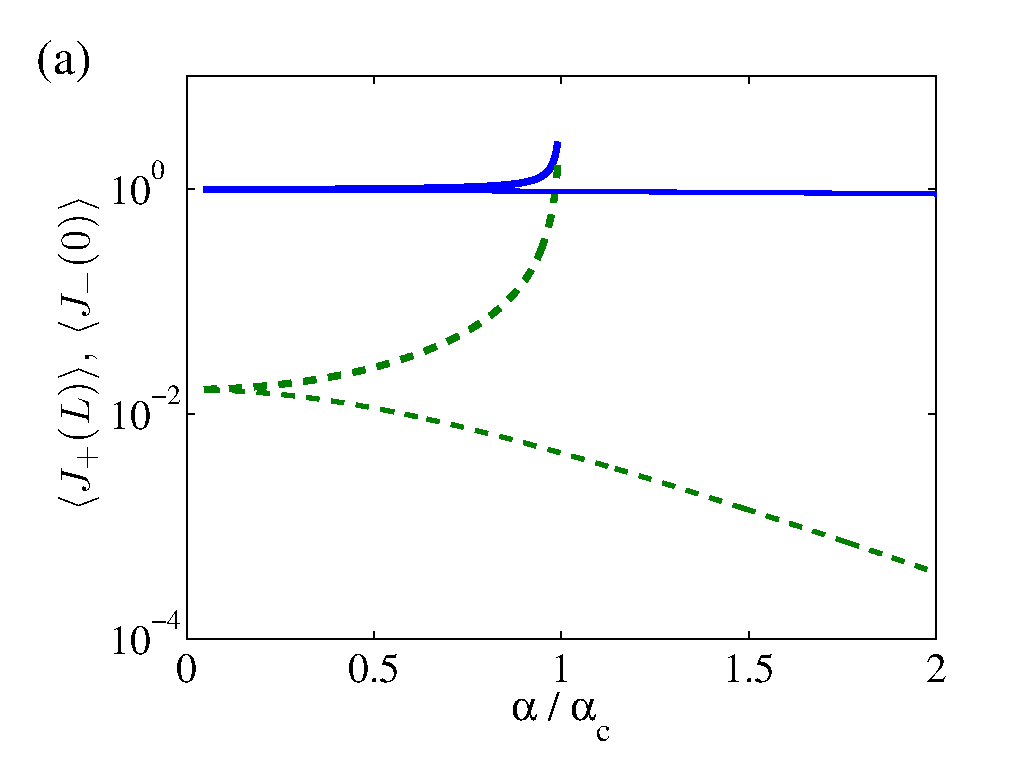
\includegraphics[width=4.5in]{chapters/paper1_asdf/pictures/fig1a_yamilov_fixed_L_variable_gain_R_T}}}
\centerline{\rotatebox{0}{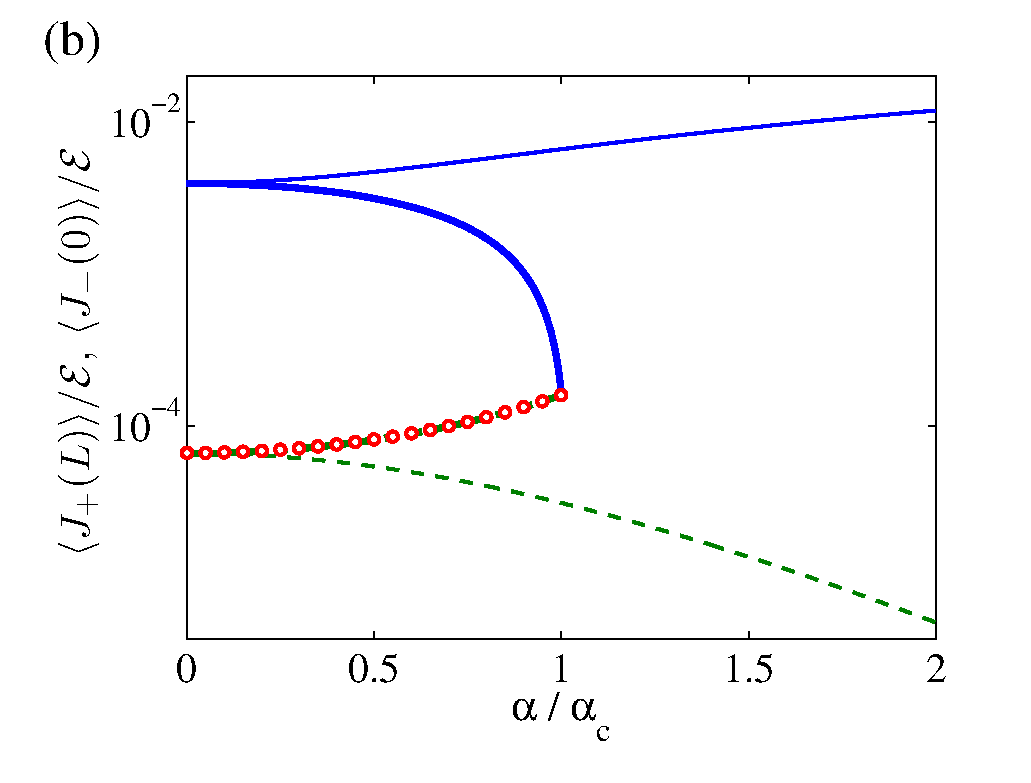
\includegraphics[width=4.5in]{chapters/paper1_asdf/pictures/fig1b_yamilov_fixed_L_variable_gain_R_T_divided_by_Energy}}}
\caption[(a) Transmission $ \langle J_{+}(L)\rangle $ (dashed line) and reflection $ \langle J_{-}(0)\rangle$ (solid line) given by Eqs.~(\ref{eq:Jreflectionflux},\ref{eq:Jtransmissionflux}) are plotted for increasing gain (thick lines) and absorption (thin lines) coefficients for a slab of random medium of thickness $L/\ell =100$.]{(a) Transmission $ \langle J_{+}(L)\rangle $ (dashed line) and reflection $ \langle J_{-}(0)\rangle$ (solid line) given by Eqs.~(\ref{eq:Jreflectionflux},\ref{eq:Jtransmissionflux}) are plotted for increasing gain (thick lines) and absorption (thin lines) coefficients for a slab of random medium of thickness $L/\ell =100$. In panel (b) we plot the same quantities as in (a) but normalized by the value of total energy stored inside random medium ${\cal E}$, c.f.~Eq.~(\ref{eq:diffusive_energy}). The divergence in the vicinity of RLT is prevented as both curves approach the same limiting value given by Eq.~(\ref{eq:Jflux_energy_constraint_cr}). $T/{\cal E}$ obtained by evaluating the approximate expression Eq.~(\ref{eq:TE_analytical}) is shown with open circles. For the chosen $L/\ell=100\gg1$ the deviation from the exact result is indiscernible.
\label{fig:diffusive_TE_ab}}
\end{figure}

\begin{figure}
\centerline{\rotatebox{0}{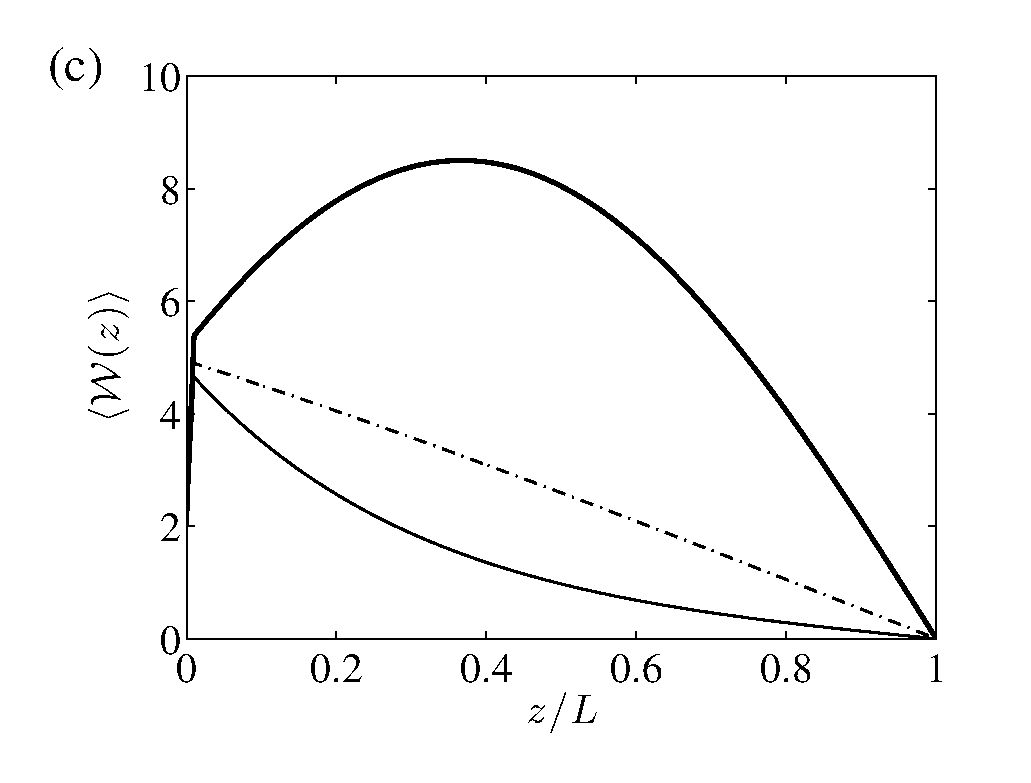
\includegraphics[width=3in]{chapters/paper1_asdf/pictures/fig1c_yamilov_diffusive_intensity_distribution}}}
\vskip -.5cm
\caption[Diffuse energy density distribution $\langle {\cal W}(z)\rangle$ inside the slab of random medium with thickness $L/\ell=100$ from Eq.~(\ref{eq:diffusive_energy}).]{Diffuse energy density distribution $\langle {\cal W}(z)\rangle$ inside the slab of random medium with thickness $L/\ell=100$ from Eq.~(\ref{eq:diffusive_energy}). Thick solid line corresponds to the sample with gain ($\alpha/\alpha_{cr}=0.8$), dashed line -- to passive sample, whereas thin solid line -- to the sample with absorption($\left|\alpha/\alpha_{cr}\right|=1$). Absorption curve is shown for comparison.
\label{fig:diffusive_TE_c}}
\end{figure}
%%%%%%%%%%%%%%%%%%%%%%%%%%%%%%%%%%%%%%%

In Fig.~\ref{fig:diffusive_TE_ab}a,b we plot Eqs.~(\ref{eq:Jreflectionflux},\ref{eq:Jtransmissionflux},\ref{eq:diffusive_energy}) for a slab of thickness $L/\ell=100$. As expected, we observe the divergence of the transmission and reflection fluxes, c.f.~Fig.~\ref{fig:diffusive_TE_ab}a, when diffusive random lasing threshold (RLT) is approached ($\alpha\rightarrow\alpha_{cr}=\pi/(L+2z_0)\simeq \pi/L$) with an increase of gain parameter $\alpha$ or, equivalently, a decrease of gain length $l_g$ toward $l_{g,cr}\simeq 3L^2/(\pi^2\ell)$. The asymptotic dependence is then
\begin{equation}
\langle J_- (0)\rangle \simeq \langle J_+ (L)\rangle \simeq J_0\frac{z_0 +
z_p}{\pi} \frac{\alpha_{cr} ^2}{\alpha_{cr} -\alpha}.
\label{eq:tr_near_threshold}
\end{equation}
Lorem ipsum dolor sit amet, consectetur adipiscing elit; Maecenas ultrices egestas commodo$L$ is increased towards critical length, $L_{cr}(\alpha)$,while keeping the gain parameter $\alpha$ fixed.

In Fig.~\ref{fig:diffusive_TE_ab}Lorem ipsum dolor sit amet, consectetur adipiscing elit; Maecenas ultrices egestas commodo$\langle J_- (0)\rangle /{\cal E}\equiv J_0R/{\cal E}$ and transmission to energy $\langle J_+ (L)\rangle /{\cal E}\equiv J_0T/{\cal E}$ obtained from Eqs.~(\ref{eq:Jreflectionflux},\ref{eq:Jtransmissionflux},\ref{eq:diffusive_energy}). One can observe that both $R/{\cal E}$ and $T/{\cal E}$ indeed remain finite at $\alpha_{cr}$Lorem ipsum dolor sit amet, consectetur adipiscing elit; Maecenas ultrices egestas commodo.~(\ref{eq:Jflux_energy_constraint_cr}). Lorem ipsum dolor sit amet, consectetur adipiscing elit; Maecenas ultrices egestas commodo$(\alpha_{cr} -\alpha )$, Eq.~(\ref{eq:tr_near_threshold}),Lorem ipsum dolor sit amet, consectetur adipiscing elit; Maecenas ultrices egestas commodo, the second order terms (not shown) are not. This explains different slopes of $R/{\cal E}$ and $T/{\cal E}$ in approach to lasing threshold in Fig.~\ref{fig:diffusive_TE}b.

By making assumption that $\ell/L\ll 1$,Lorem ipsum dolor sit amet, consectetur adipiscing elit; Maecenas ultrices egestas commodo$T/{\cal E}$ with {\it an arbitrary value of gain parameter} $\alpha$: 
\begin{equation}
\frac{T}{{\cal E}} \simeq \displaystyle\frac{D_0\alpha^2}{2J_0\sin^2\left(\alpha L/2\right)}.
\label{eq:TE_analytical}
\end{equation}
Fig.~\ref{fig:diffusive_TE_ab}Lorem ipsum dolor sit amet, consectetur adipiscing elit; Maecenas ultrices egestas commodo(open circles) Lorem ipsum dolor sit amet, consectetur adipiscing elit; Maecenas ultrices egestas commodo.~(\ref{eq:Jtransmissionflux},\ref{eq:diffusive_energy}). Lorem ipsum dolor sit amet, consectetur adipiscing elit; Maecenas ultrices egestas commodo$T/{\cal E}$ Eqs.~(\ref{eq:TE_vs_D_simple},\ref{eq:Jflux_energy_constraint_cr}) Lorem ipsum dolor sit amet, consectetur adipiscing elit; Maecenas ultrices egestas commodo.

%Lorem ipsum dolor sit amet, consectetur adipiscing elit; Maecenas ultrices egestas commodo$\langle R \rangle / \langle{\cal E}\rangle$  and $\langle T \rangle / \langle{\cal E}\rangle$. 

Based on our observations above,Lorem ipsum dolor sit amet, consectetur adipiscing elit; Maecenas ultrices egestas commodo.~\ref{sec:localization_passive}:\\
(a) Lorem ipsum dolor sit amet, consectetur adipiscing elit; Maecenas ultrices egestas commodo,Lorem ipsum dolor sit amet, consectetur adipiscing elit; Maecenas ultrices egestas commodo, c.f.~Eq.~(\ref{eq:tr_near_threshold}). Lorem ipsum dolor sit amet, consectetur adipiscing elit; Maecenas ultrices egestas commodo, without relying on the incident flux;\\
(b) Lorem ipsum dolor sit amet, consectetur adipiscing elit; Maecenas ultrices egestas commodo.~(\ref{eq:Energy_definition}), both $R/{\cal E}$  and $T/{\cal E}$Lorem ipsum dolor sit amet, consectetur adipiscing elit; Maecenas ultrices egestas commodo. Instead, they converge to the finite value of $c/(2l_{g,cr})\equiv 2D_0/L^2\times (\pi^2/4)$, c.f.~Eq.~(\ref{eq:Jflux_energy_constraint_cr}). Lorem ipsum dolor sit amet, consectetur adipiscing elit; Maecenas ultrices egestas commodo$\pi^2/4\simeq 2.5$Lorem ipsum dolor sit amet, consectetur adipiscing elit; Maecenas ultrices egestas commodo,~c.f.~Eq.~(\ref{eq:TE_vs_D_simple});\\
(c) The change of the quantities $R/{\cal E}$ and $T /{\cal E}$Lorem ipsum dolor sit amet, consectetur adipiscing elit; Maecenas ultrices egestas commodo, c.f.~Fig.~\ref{fig:diffusive_TE}c. When energy density $\langle {\cal W}(z)\rangle$Lorem ipsum dolor sit amet, consectetur adipiscing elit; Maecenas ultrices egestas commodo$\langle {\cal W}(z)\rangle\propto\sin(\pi z/L)$ the ratios $R/{\cal E}$  and $T/{\cal E}$ saturate;\\
(d) In Sec.~\ref{sec:diffusion_zero_gain} we showed, c.f.~Eq.~(\ref{eq:TE_vs_D}),Lorem ipsum dolor sit amet, consectetur adipiscing elit; Maecenas ultrices egestas commodo$T/{\cal E}$ smaller then its diffusion prediction, Eq.~(\ref{eq:TE_vs_D_simple}). Lorem ipsum dolor sit amet, consectetur adipiscing elit; Maecenas ultrices egestas commodo. Thus, Eq.~(\ref{eq:TE_analytical}) Lorem ipsum dolor sit amet, consectetur adipiscing elit; Maecenas ultrices egestas commodo,Lorem ipsum dolor sit amet, consectetur adipiscing elit; Maecenas ultrices egestas commodo.

Lorem ipsum dolor sit amet, consectetur adipiscing elit; Maecenas ultrices egestas commodo,Lorem ipsum dolor sit amet, consectetur adipiscing elit; Maecenas ultrices egestas commodo:\\
(i) The diffusion approximation (Lorem ipsum dolor sit amet, consectetur adipiscing elit; Maecenas ultrices egestas commodo) Lorem ipsum dolor sit amet, consectetur adipiscing elit; Maecenas ultrices egestas commodo. Lorem ipsum dolor sit amet, consectetur adipiscing elit; Maecenas ultrices egestas commodo;\\
(ii) Lorem ipsum dolor sit amet, consectetur adipiscing elit; Maecenas ultrices egestas commodo\cite{2005_Yamilov_correlations} and random lasing threshold \cite{1995_zyuzin_fluctuations}. Thus $T/{\cal E}$ in the form of a ratio between the {\it average}Lorem ipsum dolor sit amet, consectetur adipiscing elit; Maecenas ultrices egestas commodo$\tilde{T}$ and energy-stored $\tilde{\cal E}$ in any given realization. Instead, it may need to be replaced with $\langle \tilde{T}/\tilde{\cal E}\rangle$Lorem ipsum dolor sit amet, consectetur adipiscing elit; Maecenas ultrices egestas commodo;\\
(iii) Lorem ipsum dolor sit amet, consectetur adipiscing elit; Maecenas ultrices egestas commodo, the divergence of fluctuations of $\tilde{T}$Lorem ipsum dolor sit amet, consectetur adipiscing elit; Maecenas ultrices egestas commodo$\left\langle \left(\tilde{T}/\tilde{\cal E}\right)^n\right\rangle$ or, perhaps, its entire distribution; \\
(iv) At the onset of random lasing, nonlinear and dynamical processes\cite{2005_Cao,2009_Deych_random_laser_theory,2008_Stone,2008_Conti_opals,2009_Frank}Lorem ipsum dolor sit amet, consectetur adipiscing elit; Maecenas ultrices egestas commodo, thus, a CW quantity such as $T/{\cal E}$ may no longer be suitable.

%%%%%%%%%%%%%%%%%%%%%%%%%%%%%%%%%%%%%%%%%%%%%%%%%%%%%%%%%
\section{ANALYSIS OF \texorpdfstring{$T/{\cal E}$}{T/E}: LOCALIZED REGIME}
\label{sec:localization_passive}
%%%%%%%%%%%%%%%%%%%%%%%%%%%%%%%%%%%%%%%%%%%%%%%%%%%%%%%%%

%%%%%%%%%%%%%%%%%%%%%%%%%%%%%%%%%%%%%%%%%%%%%%%%%%%%%%%%%
\subsection{Model Description}
\label{sec:numerical_model}
%%%%%%%%%%%%%%%%%%%%%%%%%%%%%%%%%%%%%%%%%%%%%%%%%%%%%%%%%

Lorem ipsum dolor sit amet, consectetur adipiscing elit; Maecenas ultrices egestas commodo(i-iii) from Sec.~\ref{sec:diffusion_general} influence $\tilde{T}/\tilde{\cal E}$. Lorem ipsum dolor sit amet, consectetur adipiscing elit; Maecenas ultrices egestas commodo$T$ and ${\cal E}$ are reserved for the ensemble-averaged quantities. Compared to Sec.~\ref{sec:diffusion_section}, we consider the other extreme case -- the regime of localized transport --Lorem ipsum dolor sit amet, consectetur adipiscing elit; Maecenas ultrices egestas commodo. For this purpose a one-dimensional (1D) model is already sufficient. Indeed, long enough 1Lorem ipsum dolor sit amet, consectetur adipiscing elit; Maecenas ultrices egestas commodo, therefore,Lorem ipsum dolor sit amet, consectetur adipiscing elit; Maecenas ultrices egestas commodo. Despite the reduced dimensionality,Lorem ipsum dolor sit amet, consectetur adipiscing elit; Maecenas ultrices egestas commodo\cite{2006_Genack_1d,2006_Scales,2008_LunaAcosta,2005_Genack_Milner} for which the considered one-Lorem ipsum dolor sit amet, consectetur adipiscing elit; Maecenas ultrices egestas commodo.

Lorem ipsum dolor sit amet, consectetur adipiscing elit; Maecenas ultrices egestas commodo($\epsilon =$ 1 and 1.2), and width $a$. %, c.f.~Fig.~\ref{fig:dimaSetup}. 
% NOTE: fig:dimaSetup is commented out
Lorem ipsum dolor sit amet, consectetur adipiscing elit; Maecenas ultrices egestas commodo1000 pairs. One last $\epsilon = 1$Lorem ipsum dolor sit amet, consectetur adipiscing elit; Maecenas ultrices egestas commodo2001 layers. Then the total sample has length L. Lorem ipsum dolor sit amet, consectetur adipiscing elit; Maecenas ultrices egestas commodo$\epsilon=1.2$ layer. Lorem ipsum dolor sit amet, consectetur adipiscing elit; Maecenas ultrices egestas commodo($a\ll\xi$); the localization length $\xi\sim L/5$ to $L/10$,Lorem ipsum dolor sit amet, consectetur adipiscing elit; Maecenas ultrices egestas commodo\cite{2000_Deych_sps}. Lorem ipsum dolor sit amet, consectetur adipiscing elit; Maecenas ultrices egestas commodo.

Lorem ipsum dolor sit amet, consectetur adipiscing elit; Maecenas ultrices egestas commodo. Lorem ipsum dolor sit amet, consectetur adipiscing elit; Maecenas ultrices egestas commodo,Lorem ipsum dolor sit amet, consectetur adipiscing elit; Maecenas ultrices egestas commodo:
\begin{eqnarray}
&\left\{
\begin{array}{l l}
E_L(x<0,\omega)=\exp[i\omega x/c]+r_L(\omega)\exp[-i\omega x/c]\\
E_L(x>L,\omega)=t_L(\omega)\exp[i\omega x/c]\\
\end{array} \right. \label{eq:basis_functions_bc_l}\\
&\left\{
\begin{array}{l l}
E_R(x<0,\omega)=t_R(\omega)\exp[-i\omega x/c]\\
E_R(x>L,\omega)=\exp[-i\omega x/c]+r_R(\omega)\exp[i\omega x/c]\\
\end{array} \right. \label{eq:basis_functions_bc_r}
\end{eqnarray}
Here, $r_{L,R}(\omega),t_{L,R}(\omega)$Lorem ipsum dolor sit amet, consectetur adipiscing elit; Maecenas ultrices egestas commodo; $\tilde{T}=\left|t\right|^2$ and $\tilde{R}=\left|r\right|^2$. Lorem ipsum dolor sit amet, consectetur adipiscing elit; Maecenas ultrices egestas commodo$2\times 2$ transfer matrices\cite{1994_Pendry,2005_Yeh_book,2004_Mello_Kumar_book} 
\begin{equation}
\widehat{t}_i=\left[
\begin{array}{cc}
\cos(k n_i a_i) & n_i^{-1}\sin(k n_i a_i) \\
-n_i \sin(k n_i a_i) & \cos(k n_i a_i)
\end{array}
\right]
\label{eq:transfer_matrix}
\end{equation}
which act on the two-Lorem ipsum dolor sit amet, consectetur adipiscing elit; Maecenas ultrices egestas commodo. Here $n_i=\epsilon_i^{1/2}$ is the refractive index and $a_i$ is the width of the $i'$th slab.

Lorem ipsum dolor sit amet, consectetur adipiscing elit; Maecenas ultrices egestas commodo. Fig.~\ref{fig:electricFieldInSample}Lorem ipsum dolor sit amet, consectetur adipiscing elit; Maecenas ultrices egestas commodo${\cal E}$ obtained in a single realization. Subsequently,Lorem ipsum dolor sit amet, consectetur adipiscing elit; Maecenas ultrices egestas commodo. In sections~\ref{sec:correlation_te}-\ref{sec:spectral_te} the system is assumed to be passive. Lorem ipsum dolor sit amet, consectetur adipiscing elit; Maecenas ultrices egestas commodo~\ref{sec:localization_gain}.

%%%%%%%%%%%%%%%%%%%%%%%%%%%%%%%%%%%%%%%
\begin{figure}
\centerline{\rotatebox{0}{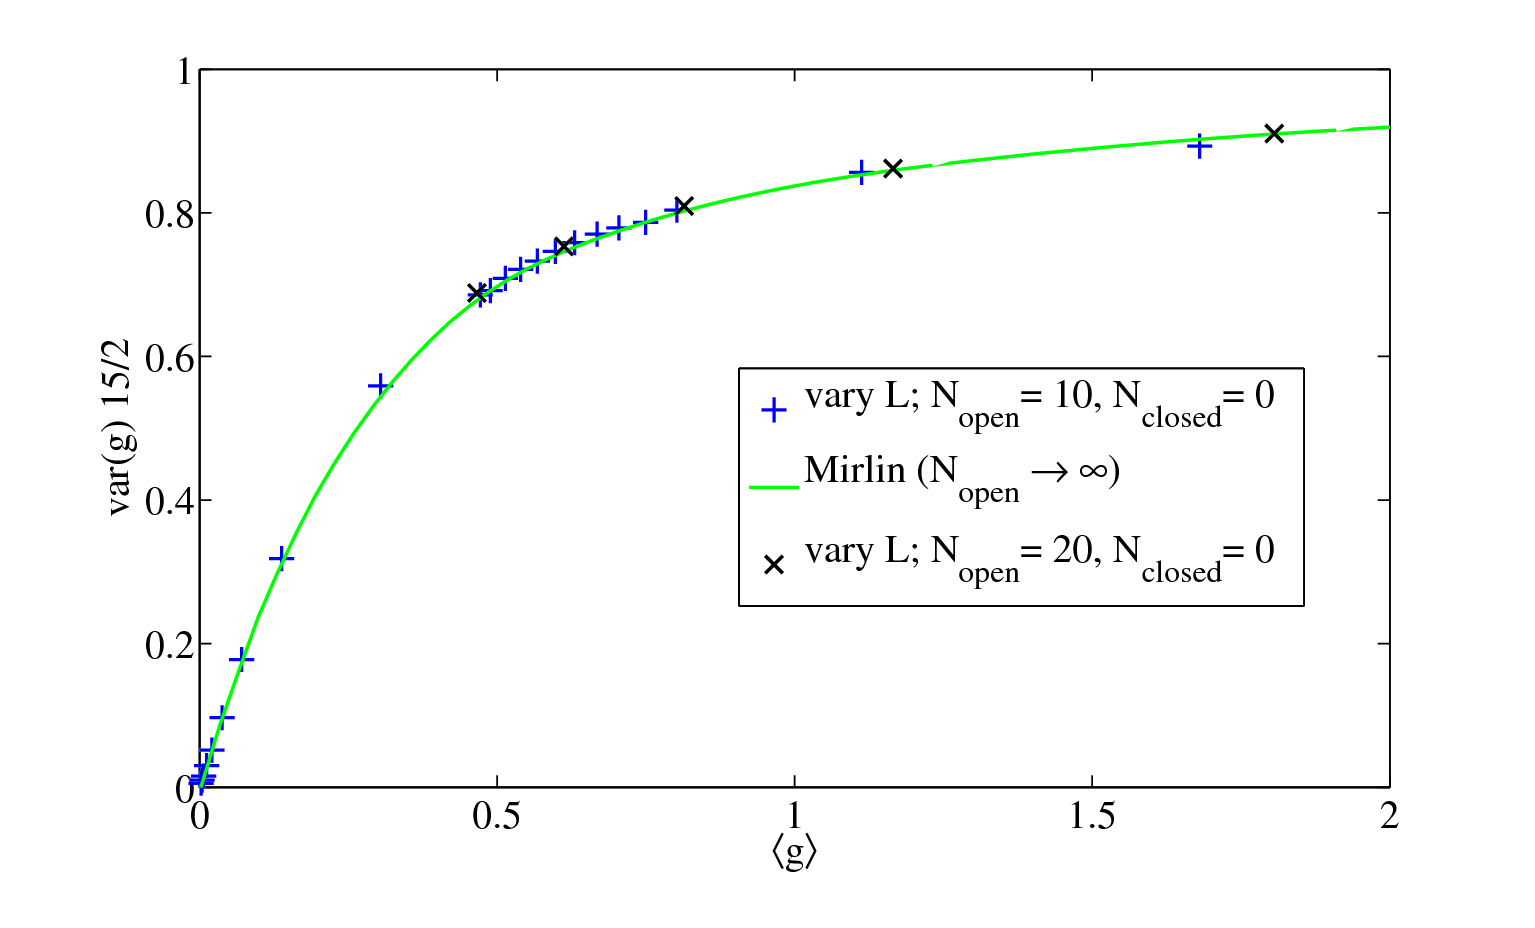
\includegraphics[width=3.5in]{pictures/var_g_versus_g_no_closed_channels}}}
\centerline{\rotatebox{0}{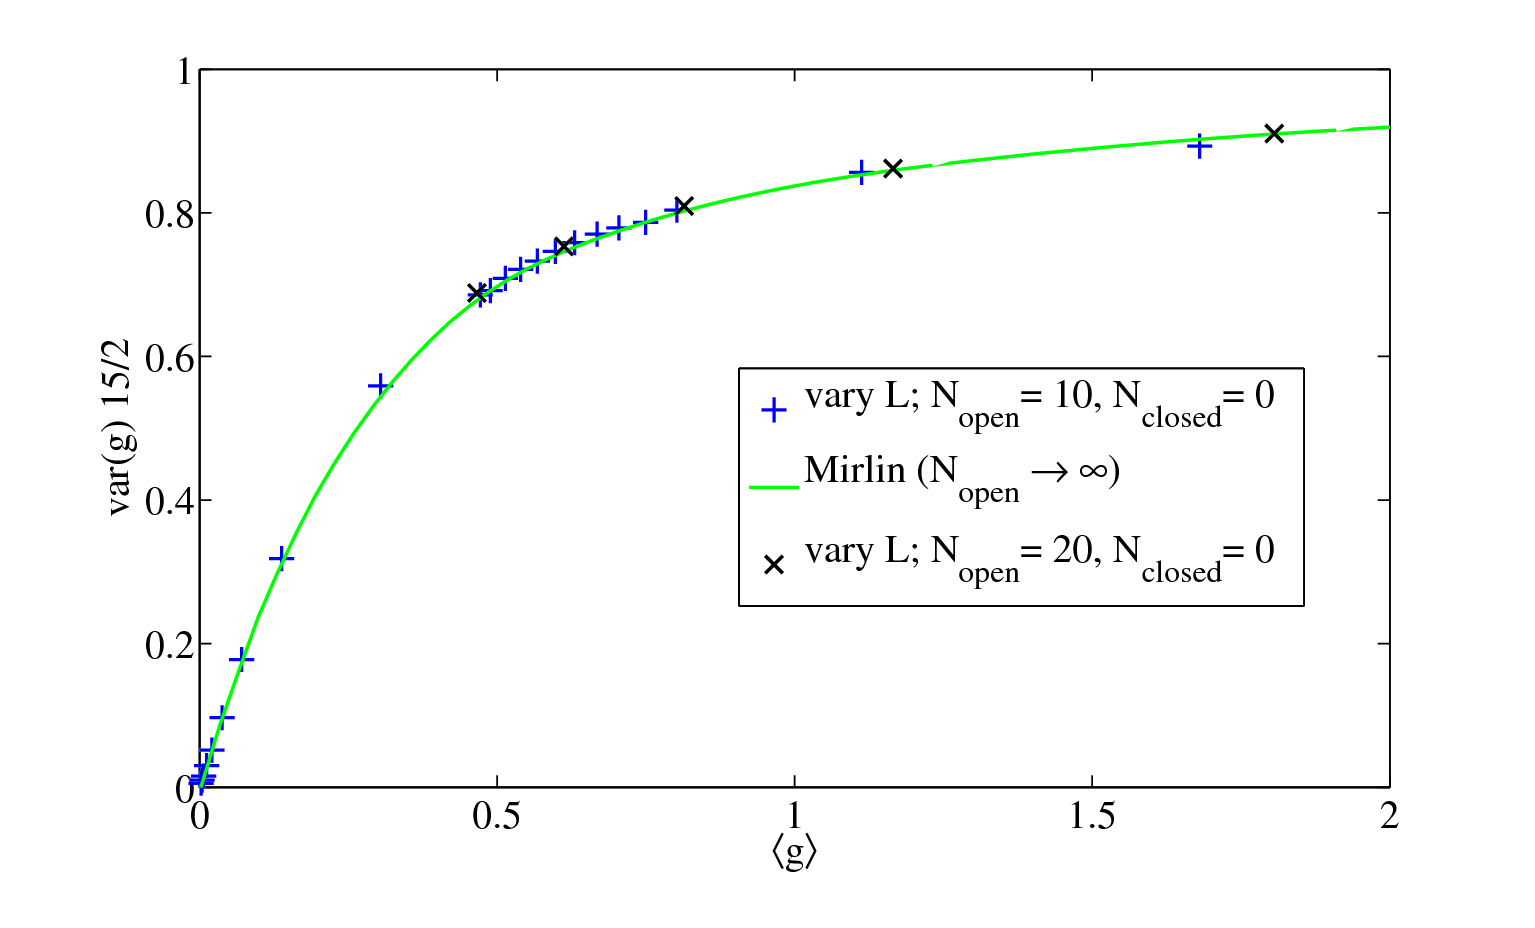
\includegraphics[width=3.5in]{pictures/var_g_versus_g_no_closed_channels}}}
%\begin{flushleft}(a)\end{flushleft}
%\vskip -0.2in
%\scalebox{0.35}{\includegraphics{pictures/tenk_energy_transmission_v_freq}}
%\begin{flushleft}(b)\end{flushleft}
%\vskip -0.1in
%\scalebox{0.38}{\includegraphics{pictures/electric_field_in_sample}}
\caption[(a) The spatially-Lorem ipsum dolor sit amet, consectetur adipiscing elit; Maecenas ultrices egestas commodo. Lorem ipsum dolor sit amet, consectetur adipiscing elit; Maecenas ultrices egestas commodo.]{
(a) The spatially-Lorem ipsum dolor sit amet, consectetur adipiscing elit; Maecenas ultrices egestas commodo. Lorem ipsum dolor sit amet, consectetur adipiscing elit; Maecenas ultrices egestas commodo. 
(b) Transmission (solid line, right $y$-axis) as a function of frequency, $\tilde{T}(\omega)$, is compared to the total energy (dashed line, left $y$-axis) in the sample $\tilde{\cal E}(\omega)$ for one random realization of disorder. No one-to-Lorem ipsum dolor sit amet, consectetur adipiscing elit; Maecenas ultrices egestas commodo.
\label{fig:electricFieldInSample}
}
\end{figure}
%%%%%%%%%%%%%%%%%%%%%%%%%%%%%%%%%%%%%%%

%%%%%%%%%%%%%%%%%%%%%%%%%%%%%%%%%%%%%%%%%%%%%%%%%%%%%%%%%
\subsection{Correlations Between \texorpdfstring{$\tilde{T}$}{T} and \texorpdfstring{$\tilde{\cal E}$}{E}}
\label{sec:correlation_te}
%%%%%%%%%%%%%%%%%%%%%%%%%%%%%%%%%%%%%%%%%%%%%%%%%%%%%%%%%

Motivated by our analysis in Section~\ref{sec:diffusion_general},Lorem ipsum dolor sit amet, consectetur adipiscing elit; Maecenas ultrices egestas commodo-model. Fig.~(\ref{fig:electricFieldInSample}b) shows $\tilde{T}$ and $\tilde{\cal E}$Lorem ipsum dolor sit amet, consectetur adipiscing elit; Maecenas ultrices egestas commodo. Lorem ipsum dolor sit amet, consectetur adipiscing elit; Maecenas ultrices egestas commodo. Indeed,Lorem ipsum dolor sit amet, consectetur adipiscing elit; Maecenas ultrices egestas commodo,Lorem ipsum dolor sit amet, consectetur adipiscing elit; Maecenas ultrices egestas commodo. Lorem ipsum dolor sit amet, consectetur adipiscing elit; Maecenas ultrices egestas commodo$\tilde{T}/\tilde{\cal E}$. Lorem ipsum dolor sit amet, consectetur adipiscing elit; Maecenas ultrices egestas commodo.

Lorem ipsum dolor sit amet, consectetur adipiscing elit; Maecenas ultrices egestas commodo. At the off-Lorem ipsum dolor sit amet, consectetur adipiscing elit; Maecenas ultrices egestas commodo. Lorem ipsum dolor sit amet, consectetur adipiscing elit; Maecenas ultrices egestas commodo,Lorem ipsum dolor sit amet, consectetur adipiscing elit; Maecenas ultrices egestas commodo. They are illustrated in Fig.~\ref{fig:Efield_random}.

In the first scenario, c.f.~bold line in Fig.~\ref{fig:Efield_random},Lorem ipsum dolor sit amet, consectetur adipiscing elit; Maecenas ultrices egestas commodo$x_0$ and falls off after it. Lorem ipsum dolor sit amet, consectetur adipiscing elit; Maecenas ultrices egestas commodo. Such behavior is attributed\cite{1983_Azbel_zeroTemp}Lorem ipsum dolor sit amet, consectetur adipiscing elit; Maecenas ultrices egestas commodo$x_0$. 

In the other case, c.f.~thin line in Fig.~\ref{fig:Efield_random},Lorem ipsum dolor sit amet, consectetur adipiscing elit; Maecenas ultrices egestas commodo(Lorem ipsum dolor sit amet, consectetur adipiscing elit; Maecenas ultrices egestas commodo, see figure caption). Lorem ipsum dolor sit amet, consectetur adipiscing elit; Maecenas ultrices egestas commodo,Lorem ipsum dolor sit amet, consectetur adipiscing elit; Maecenas ultrices egestas commodo$\tilde{\cal E}$. Lorem ipsum dolor sit amet, consectetur adipiscing elit; Maecenas ultrices egestas commodo.~\ref{fig:Efield_random} were studied in Ref. \cite{1983_Azbel_zeroTemp},Lorem ipsum dolor sit amet, consectetur adipiscing elit; Maecenas ultrices egestas commodo.~\ref{fig:Efield_random}Lorem ipsum dolor sit amet, consectetur adipiscing elit; Maecenas ultrices egestas commodo.

We note that multi-Lorem ipsum dolor sit amet, consectetur adipiscing elit; Maecenas ultrices egestas commodo-called necklace states\cite{1987_Pendry,2005_Wiersma,2006_Genack_1d}Lorem ipsum dolor sit amet, consectetur adipiscing elit; Maecenas ultrices egestas commodo(almost) Lorem ipsum dolor sit amet, consectetur adipiscing elit; Maecenas ultrices egestas commodo. Such realizations, however,Lorem ipsum dolor sit amet, consectetur adipiscing elit; Maecenas ultrices egestas commodo$L\gg\xi$Lorem ipsum dolor sit amet, consectetur adipiscing elit; Maecenas ultrices egestas commodo. 

We find that, on average,Lorem ipsum dolor sit amet, consectetur adipiscing elit; Maecenas ultrices egestas commodo$\tilde{\cal E}$. Lorem ipsum dolor sit amet, consectetur adipiscing elit; Maecenas ultrices egestas commodo,Lorem ipsum dolor sit amet, consectetur adipiscing elit; Maecenas ultrices egestas commodo.~\ref{fig:Efield_random}Lorem ipsum dolor sit amet, consectetur adipiscing elit; Maecenas ultrices egestas commodo. Indeed,Lorem ipsum dolor sit amet, consectetur adipiscing elit; Maecenas ultrices egestas commodo,Lorem ipsum dolor sit amet, consectetur adipiscing elit; Maecenas ultrices egestas commodo. Lorem ipsum dolor sit amet, consectetur adipiscing elit; Maecenas ultrices egestas commodo.~\ref{fig:Efield_random}. In contrast,Lorem ipsum dolor sit amet, consectetur adipiscing elit; Maecenas ultrices egestas commodo(or non-distinguishable) peak in energy,Lorem ipsum dolor sit amet, consectetur adipiscing elit; Maecenas ultrices egestas commodo(closer to the exit boundary). Lorem ipsum dolor sit amet, consectetur adipiscing elit; Maecenas ultrices egestas commodo.~\ref{fig:Efield_random}.\\

%%%%%%%%%%%%%%%%%%%%%%%%%%%%%%%%%%%%%%%
\begin{figure}
\centerline{\rotatebox{0}{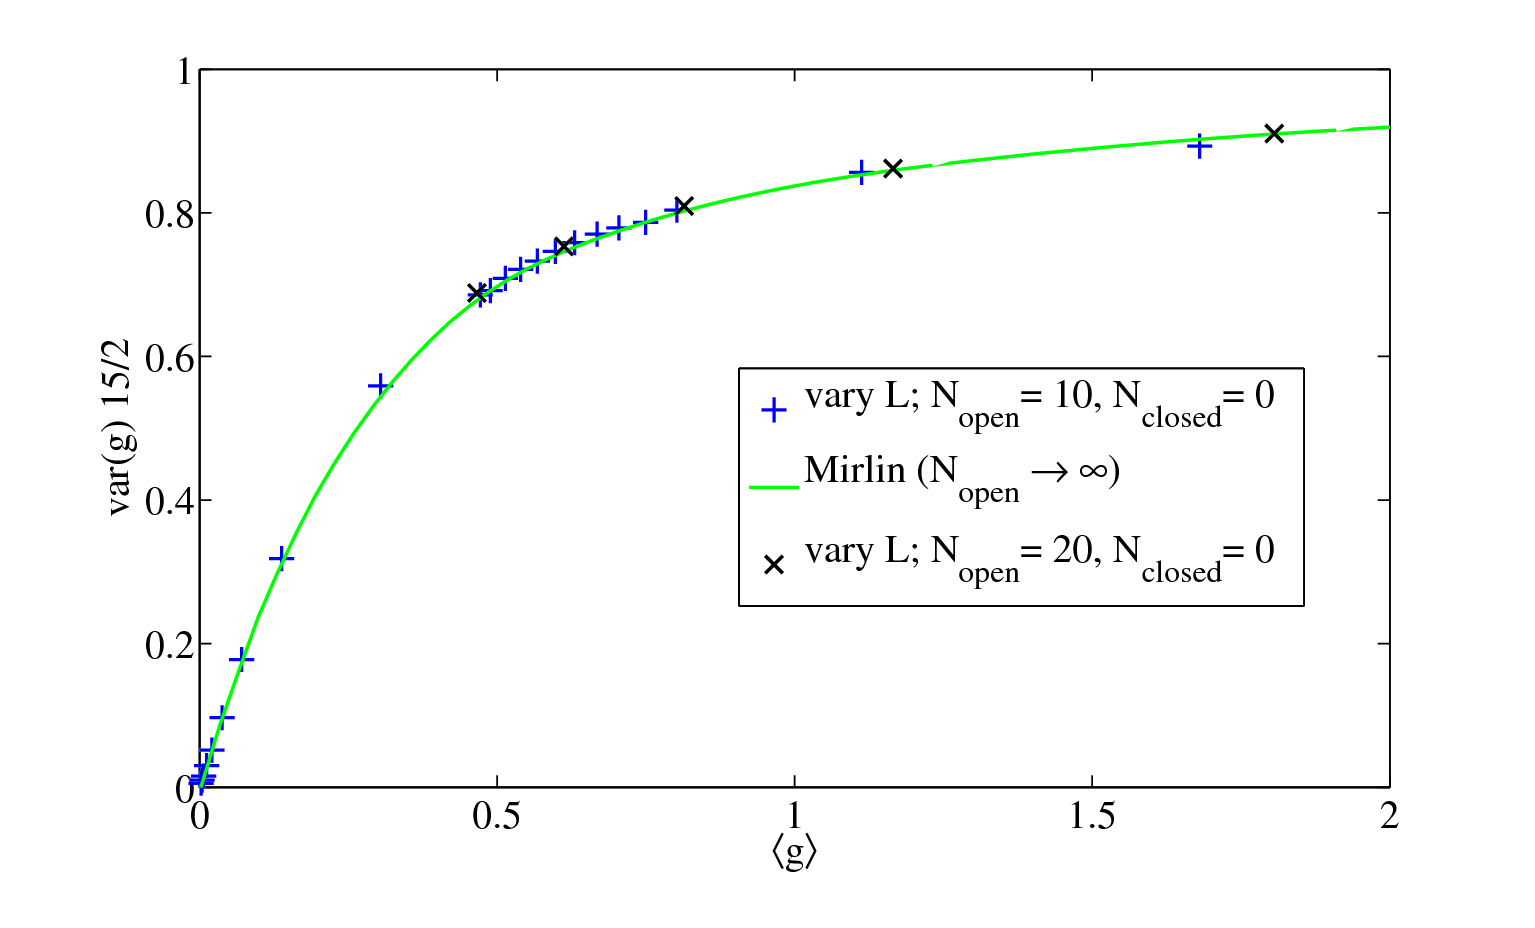
\includegraphics[width=3.25in]{pictures/var_g_versus_g_no_closed_channels}}}
%\scalebox{0.36}{\includegraphics{pictures/rlz2_elecfield_14_34.eps}}
\caption[Two types of the on-Lorem ipsum dolor sit amet, consectetur adipiscing elit; Maecenas ultrices egestas commodo$x_0$ in the first half (bold lines) and the second half (thin lines) of the sample ($x_0/L \approx 0.25$).]{
Two types of the on-Lorem ipsum dolor sit amet, consectetur adipiscing elit; Maecenas ultrices egestas commodo$x_0$ in the first half (bold lines) and the second half (thin lines) of the sample ($x_0/L \approx 0.25$). Lorem ipsum dolor sit amet, consectetur adipiscing elit; Maecenas ultrices egestas commodo,Lorem ipsum dolor sit amet, consectetur adipiscing elit; Maecenas ultrices egestas commodo.~(\ref{eq:basis_functions_bc_l}) to Eq.~(\ref{eq:basis_functions_bc_r}). Due to reciprocity,Lorem ipsum dolor sit amet, consectetur adipiscing elit; Maecenas ultrices egestas commodo. However,Lorem ipsum dolor sit amet, consectetur adipiscing elit; Maecenas ultrices egestas commodo. Lorem ipsum dolor sit amet, consectetur adipiscing elit; Maecenas ultrices egestas commodo$\tilde{\cal E}(\omega)$. Lorem ipsum dolor sit amet, consectetur adipiscing elit; Maecenas ultrices egestas commodo$\exp(\pm x/ \xi)$ spatial dependences. Lorem ipsum dolor sit amet, consectetur adipiscing elit; Maecenas ultrices egestas commodo.~\ref{sec:numerical_model}. 
\label{fig:Efield_random}}
\end{figure}
%%%%%%%%%%%%%%%%%%%%%%%%%%%%%%%%%%%%%%%

Lorem ipsum dolor sit amet, consectetur adipiscing elit; Maecenas ultrices egestas commodo,Lorem ipsum dolor sit amet, consectetur adipiscing elit; Maecenas ultrices egestas commodo. A sample with a localized state $0<x_0<L/2$ automatically yields the $L/2<x_0<L$ state in the mirror-image sample or, equivalently,Lorem ipsum dolor sit amet, consectetur adipiscing elit; Maecenas ultrices egestas commodo.~\ref{fig:Efield_random}. Lorem ipsum dolor sit amet, consectetur adipiscing elit; Maecenas ultrices egestas commodo. However,Lorem ipsum dolor sit amet, consectetur adipiscing elit; Maecenas ultrices egestas commodo, thus, energy stored, is dramatically different. In Appx.~\ref{app:qm_model}Lorem ipsum dolor sit amet, consectetur adipiscing elit; Maecenas ultrices egestas commodo. Indeed,Lorem ipsum dolor sit amet, consectetur adipiscing elit; Maecenas ultrices egestas commodo.~\ref{app:qm_model} (c.f.~Figs.~\ref{fig:Efield_random},\ref{fig:barrierdefectlog}) can be also obtained in  other models. Lorem ipsum dolor sit amet, consectetur adipiscing elit; Maecenas ultrices egestas commodo.~\ref{sec:numerical_model}, but with no disorder. Lorem ipsum dolor sit amet, consectetur adipiscing elit; Maecenas ultrices egestas commodo, appear equivalent to that in Fig.~\ref{fig:barrierdefectlog}.
 
Lorem ipsum dolor sit amet, consectetur adipiscing elit; Maecenas ultrices egestas commodo: (i) Lorem ipsum dolor sit amet, consectetur adipiscing elit; Maecenas ultrices egestas commodo($x_0$) Lorem ipsum dolor sit amet, consectetur adipiscing elit; Maecenas ultrices egestas commodo. (ii) Lorem ipsum dolor sit amet, consectetur adipiscing elit; Maecenas ultrices egestas commodo. (iii) Lorem ipsum dolor sit amet, consectetur adipiscing elit; Maecenas ultrices egestas commodo. And otherwise,Lorem ipsum dolor sit amet, consectetur adipiscing elit; Maecenas ultrices egestas commodo.

%%%%%%%%%%%%%%%%%%%%%%%%%%%%%%%%%%%%%%%%%%%%%%%%%%%%%%%%%
\subsection{Behavior of \texorpdfstring{$\tilde{T}/\tilde{\cal E}$}{T/E} in Passive Random Medium: Spectral Vicinity of a Resonance}
\label{sec:spectral_te}

%%%%%%%%%%%%%%%%%%%%%%%%%%%%%%%%%%%%%%%%%%%%%%%%%%%%%%%%%

%%%%%%%%%%%%%%%%%%%%%%%%%%%%%%%%%%%%%%%
\begin{figure*}
\vskip -0.0in
\centerline{\rotatebox{0}{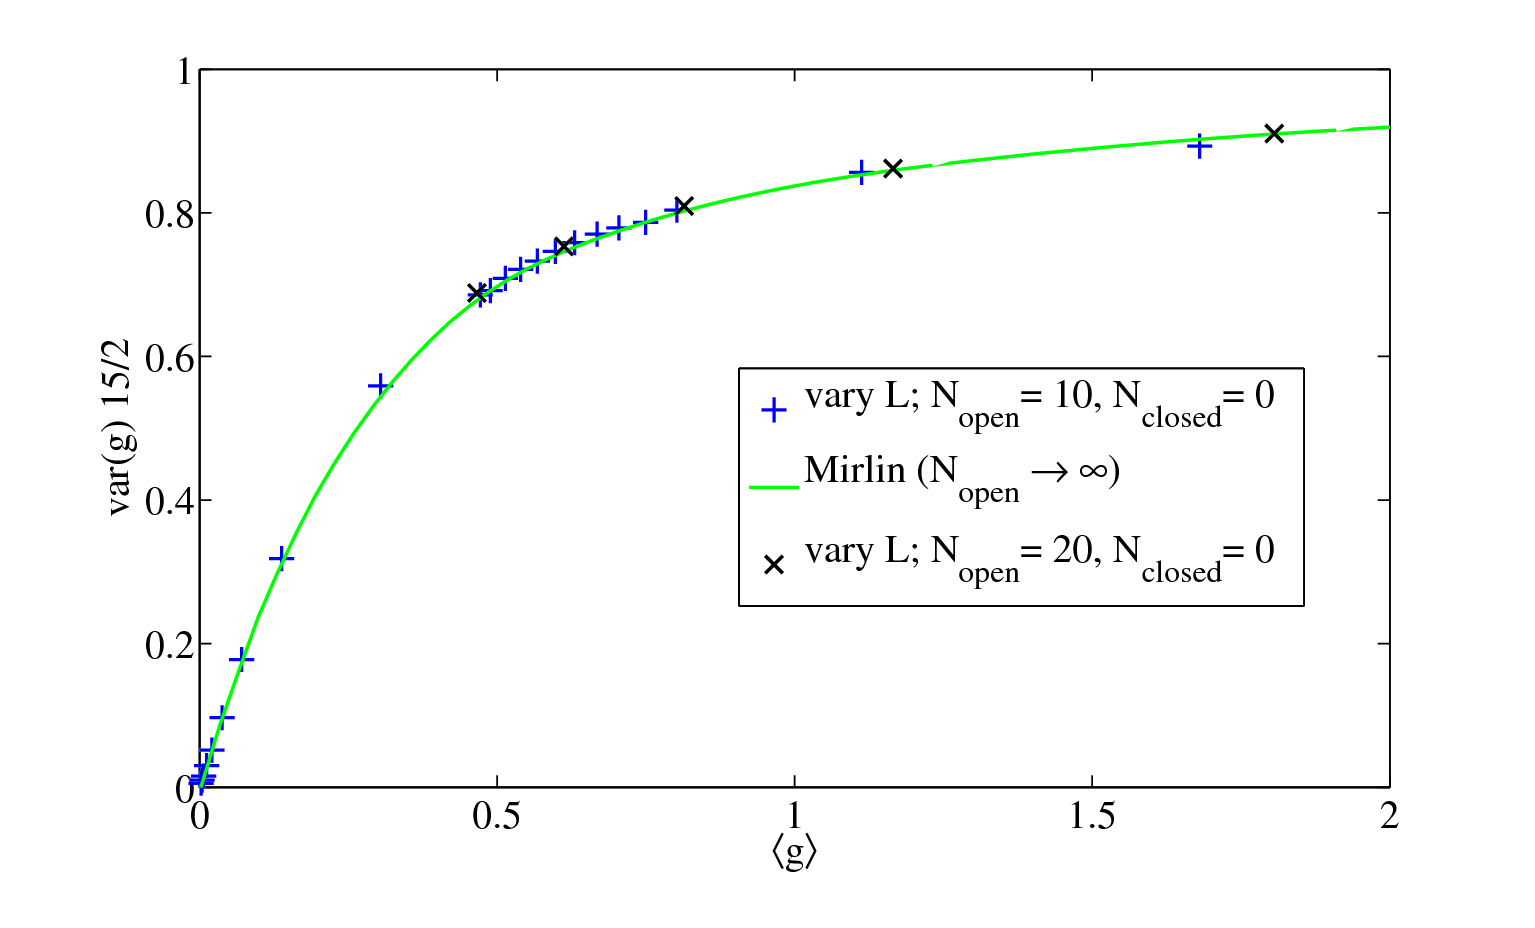
\includegraphics[width=7.5in]{pictures/var_g_versus_g_no_closed_channels}}}
%\centerline{\scalebox{0.65}{\includegraphics{pictures/peaks_match_peaks_dont_match1}}}
\vskip 0.0in
\caption[The dependencies of $\tilde{T}(\omega )$ (a,b); envelope of the electric field  $E(x)$ (c,d); and energy in the system $\tilde{\cal E}(\omega )$ (e,f).]{The dependencies of $\tilde{T}(\omega )$ (a,b); envelope of the electric field  $E(x)$ (c,d); and energy in the system $\tilde{\cal E}(\omega )$ (e,f). Lorem ipsum dolor sit amet, consectetur adipiscing elit; Maecenas ultrices egestas commodo. The plots (a,c,e) and (b,d,f) Lorem ipsum dolor sit amet, consectetur adipiscing elit; Maecenas ultrices egestas commodo$x_0=L/4$ and $x_0=3L/4$ respectively. Lorem ipsum dolor sit amet, consectetur adipiscing elit; Maecenas ultrices egestas commodo.~(\ref{eq:basis_functions_bc_r}) -- wave incident from the right -- for easy comparison with Figs.~\ref{fig:Efield_random},\ref{fig:barrierdefectlog}. In the first case,Lorem ipsum dolor sit amet, consectetur adipiscing elit; Maecenas ultrices egestas commodo. Three sets of $E(x)$ in (c,d) Lorem ipsum dolor sit amet, consectetur adipiscing elit; Maecenas ultrices egestas commodo(a,b,e,f). The envelopes illustrate the on- and off-Lorem ipsum dolor sit amet, consectetur adipiscing elit; Maecenas ultrices egestas commodo.~(\ref{eq:left},\ref{eq:right},\ref{eq:startingequations},\ref{eq:energy_stored}). Lorem ipsum dolor sit amet, consectetur adipiscing elit; Maecenas ultrices egestas commodo,Lorem ipsum dolor sit amet, consectetur adipiscing elit; Maecenas ultrices egestas commodo. In this case, unlike $\tilde{T}(\omega )$, $\tilde{\cal E}(\omega )$Lorem ipsum dolor sit amet, consectetur adipiscing elit; Maecenas ultrices egestas commodo$\omega_0$, compare (e) and (f). Lorem ipsum dolor sit amet, consectetur adipiscing elit; Maecenas ultrices egestas commodo$0<x_0<L/2$ and $L/2<x_0<L$ in the $\tilde{T}/\tilde{\cal E}$ as discussed in Sec.~\ref{sec:correlation_te} and Appx.~\ref{app:qm_model}.
\label{fig:peaksmatchnotmatch}}
\end{figure*}
%%%%%%%%%%%%%%%%%%%%%%%%%%%%%%%%%%%%%%%

Lorem ipsum dolor sit amet, consectetur adipiscing elit; Maecenas ultrices egestas commodo.~\ref{sec:correlation_te} and Appx.~\ref{app:qm_model}Lorem ipsum dolor sit amet, consectetur adipiscing elit; Maecenas ultrices egestas commodo$\tilde{T}/\tilde{\cal E}$Lorem ipsum dolor sit amet, consectetur adipiscing elit; Maecenas ultrices egestas commodo.

In the localization regime,Lorem ipsum dolor sit amet, consectetur adipiscing elit; Maecenas ultrices egestas commodo,Lorem ipsum dolor sit amet, consectetur adipiscing elit; Maecenas ultrices egestas commodo, via resonant tunneling. Thus,Lorem ipsum dolor sit amet, consectetur adipiscing elit; Maecenas ultrices egestas commodo-Lorem ipsum dolor sit amet, consectetur adipiscing elit; Maecenas ultrices egestas commodo:
\begin{equation}
\tilde{T}(\omega) = \frac{t_0^2}{\left[2(k-k_0)\Delta\right]^2+t_0^2\cosh^2\displaystyle\frac{\left|L-2x_0\right|}{\xi} }
\label{eq:transmission}
\end{equation}
where $k=\omega/c$ and $t_0=\exp(-L/\xi)$Lorem ipsum dolor sit amet, consectetur adipiscing elit; Maecenas ultrices egestas commodo$k_0$. $\Delta$Lorem ipsum dolor sit amet, consectetur adipiscing elit; Maecenas ultrices egestas commodo. Lorem ipsum dolor sit amet, consectetur adipiscing elit; Maecenas ultrices egestas commodo``cavity"\cite{2008_Bliokh}. $\Delta$Lorem ipsum dolor sit amet, consectetur adipiscing elit; Maecenas ultrices egestas commodo, see e.g. \cite{1994_Pendry,2001_Deych_mqw}. In the case of random media, $\Delta$Lorem ipsum dolor sit amet, consectetur adipiscing elit; Maecenas ultrices egestas commodo. In this system $\Delta$Lorem ipsum dolor sit amet, consectetur adipiscing elit; Maecenas ultrices egestas commodo\cite{2004_Bliokh_wavelet}.

Of course,Lorem ipsum dolor sit amet, consectetur adipiscing elit; Maecenas ultrices egestas commodo.~\ref{app:qm_model}Lorem ipsum dolor sit amet, consectetur adipiscing elit; Maecenas ultrices egestas commodo.~(\ref{eq:transmission}). However,Lorem ipsum dolor sit amet, consectetur adipiscing elit; Maecenas ultrices egestas commodo$k-k_0,x_0,\xi$ and ,$L$: Eq.~(\ref{eq:transmission}) Lorem ipsum dolor sit amet, consectetur adipiscing elit; Maecenas ultrices egestas commodo$\left|k-k_0\right|\leq\delta k$ and $L\gg\xi$ (which also leads to $\delta k\ll k_0$ condition). Here $\delta k$ is the spectral width of the resonance.

Lorem ipsum dolor sit amet, consectetur adipiscing elit; Maecenas ultrices egestas commodo1Lorem ipsum dolor sit amet, consectetur adipiscing elit; Maecenas ultrices egestas commodo.~\ref{app:qm_model} was demonstrated in Ref. \cite{2004_Bliokh_wavelet}. Therefore, we expect Eq.~(\ref{eq:transmission}) Lorem ipsum dolor sit amet, consectetur adipiscing elit; Maecenas ultrices egestas commodo.~\ref{sec:numerical_model}.

We note two important properties of Eq.~(\ref{eq:transmission}). First, the maximum (resonant) value of the transmission at $\omega =\omega_0$Lorem ipsum dolor sit amet, consectetur adipiscing elit; Maecenas ultrices egestas commodo$\tilde{T}(\omega_0)=\cosh^{-2}\left(\left|L-2x_0\right|/\xi\right)$. It turns to unity when $x_0=L/2$. Secondly,Lorem ipsum dolor sit amet, consectetur adipiscing elit; Maecenas ultrices egestas commodo$\left|\omega-\omega_0\right|\gg\delta\omega$,Lorem ipsum dolor sit amet, consectetur adipiscing elit; Maecenas ultrices egestas commodo--Lorem ipsum dolor sit amet, consectetur adipiscing elit; Maecenas ultrices egestas commodo.

%%%%%%%%%%%%%%%%%%%%%%%%%%%%%%%%%%%%%%%
\begin{figure}
\centerline{\rotatebox{0}{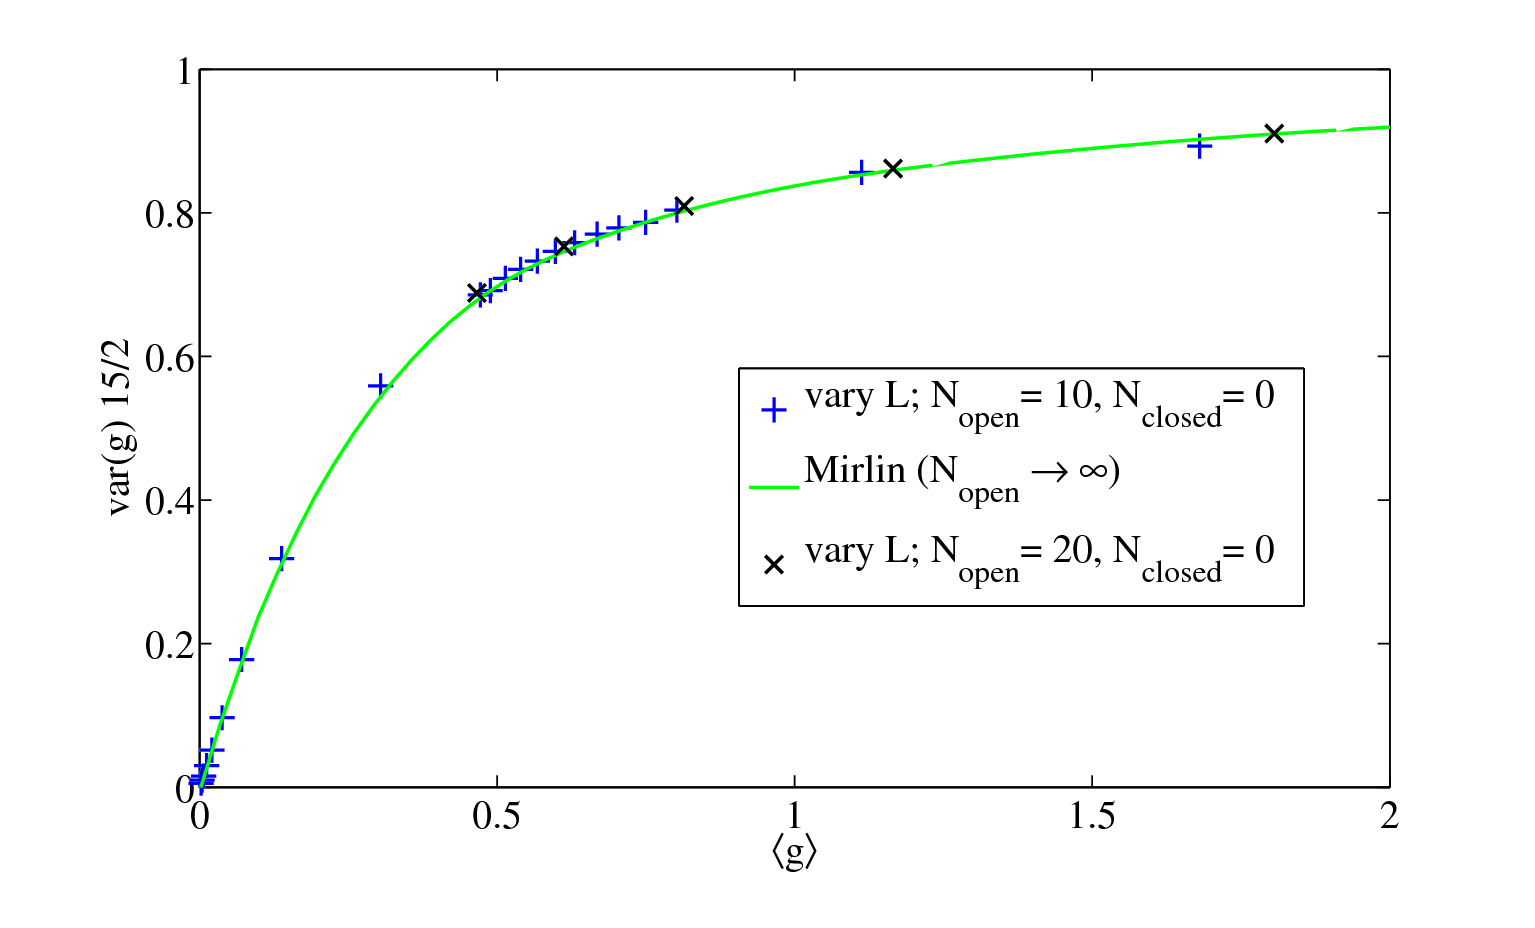
\includegraphics[width=3.5in]{pictures/var_g_versus_g_no_closed_channels}}}
%\vskip -0.0cm
%\centerline{
%\scalebox{0.5}{\includegraphics{pictures/energy_distribution_and_TE_dual_axis.eps}}}
%\vskip -0.0cm
\caption[The solid line plots $\tilde{\cal E}(\omega_0,x_0)$ from Eq.~(\ref{eq:energy_stored}).]{The solid line plots $\tilde{\cal E}(\omega_0,x_0)$ from Eq.~(\ref{eq:energy_stored}). Lorem ipsum dolor sit amet, consectetur adipiscing elit; Maecenas ultrices egestas commodo(exponentially) when the center of localization $x_0$ increases beyond $L/2$ and reaches the off-resonant value for $x_0>2L/3$. The dashed line with the right $y$-axis represents the ratio between $\tilde{T}(\omega_0,x_0)$ in Eq.~(\ref{eq:transmission}) and  $\tilde{\cal E}(\omega_0,x_0)$ in Eq.~(\ref{eq:energy_stored}). The ratio peaks at the same value of $x_0/L=2/3$. Lorem ipsum dolor sit amet, consectetur adipiscing elit; Maecenas ultrices egestas commodo$\xi$ or the system length $L$. \label{fig:energydistrib}}
\end{figure}
%%%%%%%%%%%%%%%%%%%%%%%%%%%%%%%%%%%%%%%

%\begin{widetext}
Lorem ipsum dolor sit amet, consectetur adipiscing elit; Maecenas ultrices egestas commodo.~\ref{sec:correlation_te} and Appx.~\ref{app:qm_model}, c.f.~Figs.~\ref{fig:Efield_random},\ref{fig:barrierdefectlog}, we approximate the envelope of the {\it on-resonance} electric field distribution as
\begin{equation}
E(x,\omega_0) = \left\{
\begin{array}{l l}
B(\omega_0,x_0) \exp [ (x-x_0)/\xi ] &\quad 0 < x < x_0 \\
C(\omega_0,x_0) \exp [-(x-x_0)/\xi ] &\quad x_0 < x < L\\
\end{array} \right.
\label{eq:left}
\end{equation}
for $x_0<L/2$; and
\begin{equation}
E(x,\omega_0) = \left\{
\begin{array}{l l}
 A(\omega_0,x_0) \exp [-x      /\xi ] &\quad 0 < x < x_T(\omega_0)   \\
 B(\omega_0,x_0) \exp [ (x-x_0)/\xi ] &\quad x_T(\omega_0) < x < x_0 \\
 C(\omega_0,x_0) \exp [-(x-x_0)/\xi ] &\quad x_0 < x < L \\
\end{array} \right.
\label{eq:right}
\end{equation}
for $x_0>L/2$. Here $A,B,C$Lorem ipsum dolor sit amet, consectetur adipiscing elit; Maecenas ultrices egestas commodo. At the boundaries we set $E(x=0)=1$ and $E(x=L)=\tilde{T}^{1/2}(\omega_0)$. Noticing that $E(x=L,\omega_0)\approx\exp\left[ -|2x_0-L|/\xi\right]$Lorem ipsum dolor sit amet, consectetur adipiscing elit; Maecenas ultrices egestas commodo, $x_T(\omega_0)=2x_0-L$, in the case of Eq.~(\ref{eq:right}). Lorem ipsum dolor sit amet, consectetur adipiscing elit; Maecenas ultrices egestas commodo, such as in Sec.~\ref{sec:numerical_model}, the Eqs.~(\ref{eq:left},\ref{eq:right}) Lorem ipsum dolor sit amet, consectetur adipiscing elit; Maecenas ultrices egestas commodo$(\omega-\omega_0),x_0,\xi$, and $L$.

In both cases above, away from the resonant frequency $k_0$, we see three distinct regions:
\begin{equation}
E(x) = \left\{
\begin{array}{l l}
A(\omega,x_0) \exp[- x     /\xi]  &\quad 0 < x < x_T(\omega)    \\
B(\omega,x_0) \exp[ (x-x_0)/\xi]  &\quad x_T(\omega) < x < x_0  \\
C(\omega,x_0) \exp[-(x-x_0)/\xi]  &\quad x_0 < x < L    \\
\end{array} \right. 
\label{eq:startingequations}
\end{equation}
where $x_T(\omega)$Lorem ipsum dolor sit amet, consectetur adipiscing elit; Maecenas ultrices egestas commodo$E(x=0)=1$ and $E(x=L)=T^{1/2}(\omega)$. Fig.~\ref{fig:peaksmatchnotmatch}Lorem ipsum dolor sit amet, consectetur adipiscing elit; Maecenas ultrices egestas commodo$x_0<L/2$ and $x_0>L/2$ cases. Lorem ipsum dolor sit amet, consectetur adipiscing elit; Maecenas ultrices egestas commodo$x_0$. Indeed, integrating Eqs.~(\ref{eq:left},\ref{eq:right}) gives us the sought expression for $\tilde{\cal E}(\omega)$. At $\omega=\omega_0$ it simplifies to
\begin{equation}
\tilde{\cal E}(x_0)\propto\left\{
\begin{array}{l l}
2\tilde{T}(\omega)\exp\left[2(L-x_0)/\xi\right]-1- \tilde{T}(\omega) & \quad 0  < x_0 < L/2 \\
2\tilde{T}(\omega)\exp\left[2(L-x_0)/\xi\right]+1-3\tilde{T}(\omega) & \quad L/2< x_0 < L   \\
\end{array}
\right.
\label{eq:energy_stored}
\end{equation}
%\end{widetext}
This expression is plotted in Fig.~\ref{fig:energydistrib}. Lorem ipsum dolor sit amet, consectetur adipiscing elit; Maecenas ultrices egestas commodo$x_0<L/2$ and $x_0>L/2$. Eq.~(\ref{eq:energy_stored}) Lorem ipsum dolor sit amet, consectetur adipiscing elit; Maecenas ultrices egestas commodo-resonant case for $x_0>2L/3$. The latter value of $x_0$Lorem ipsum dolor sit amet, consectetur adipiscing elit; Maecenas ultrices egestas commodo$\xi$, $L$, etc.

When expressions in Eqs.~(\ref{eq:transmission},\ref{eq:energy_stored}) are combined to form the ratio $\tilde{T}/\tilde{\cal E}$,Lorem ipsum dolor sit amet, consectetur adipiscing elit; Maecenas ultrices egestas commodo$x_0$, c.f.~Fig.~\ref{fig:energydistrib}. Lorem ipsum dolor sit amet, consectetur adipiscing elit; Maecenas ultrices egestas commodo$0<x_0<2L/3$Lorem ipsum dolor sit amet, consectetur adipiscing elit; Maecenas ultrices egestas commodo$2L/3<x_0<L$. Lorem ipsum dolor sit amet, consectetur adipiscing elit; Maecenas ultrices egestas commodo$\tilde{T}/\tilde{\cal E}$ on $x_0$. Lorem ipsum dolor sit amet, consectetur adipiscing elit; Maecenas ultrices egestas commodo(linear) optical amplification on this quantity.

%%%%%%%%%%%%%%%%%%%%%%%%%%%%%%%%%%%%%%%%%%%%%%%%%%%%%%%%%
\subsection{Behavior of \texorpdfstring{$\tilde{T}/\tilde{\cal E}$}{T/E} in Active Random Medium} 
\label{sec:localization_gain}
%%%%%%%%%%%%%%%%%%%%%%%%%%%%%%%%%%%%%%%%%%%%%%%%%%%%%%%%%

%%%%%%%%%%%%%%%%%%%%%%%%%%%%%%%%%%%%%%%%%%%%%%%%%%%%%%%%%%%%%%
\begin{figure}
\centerline{\rotatebox{0}{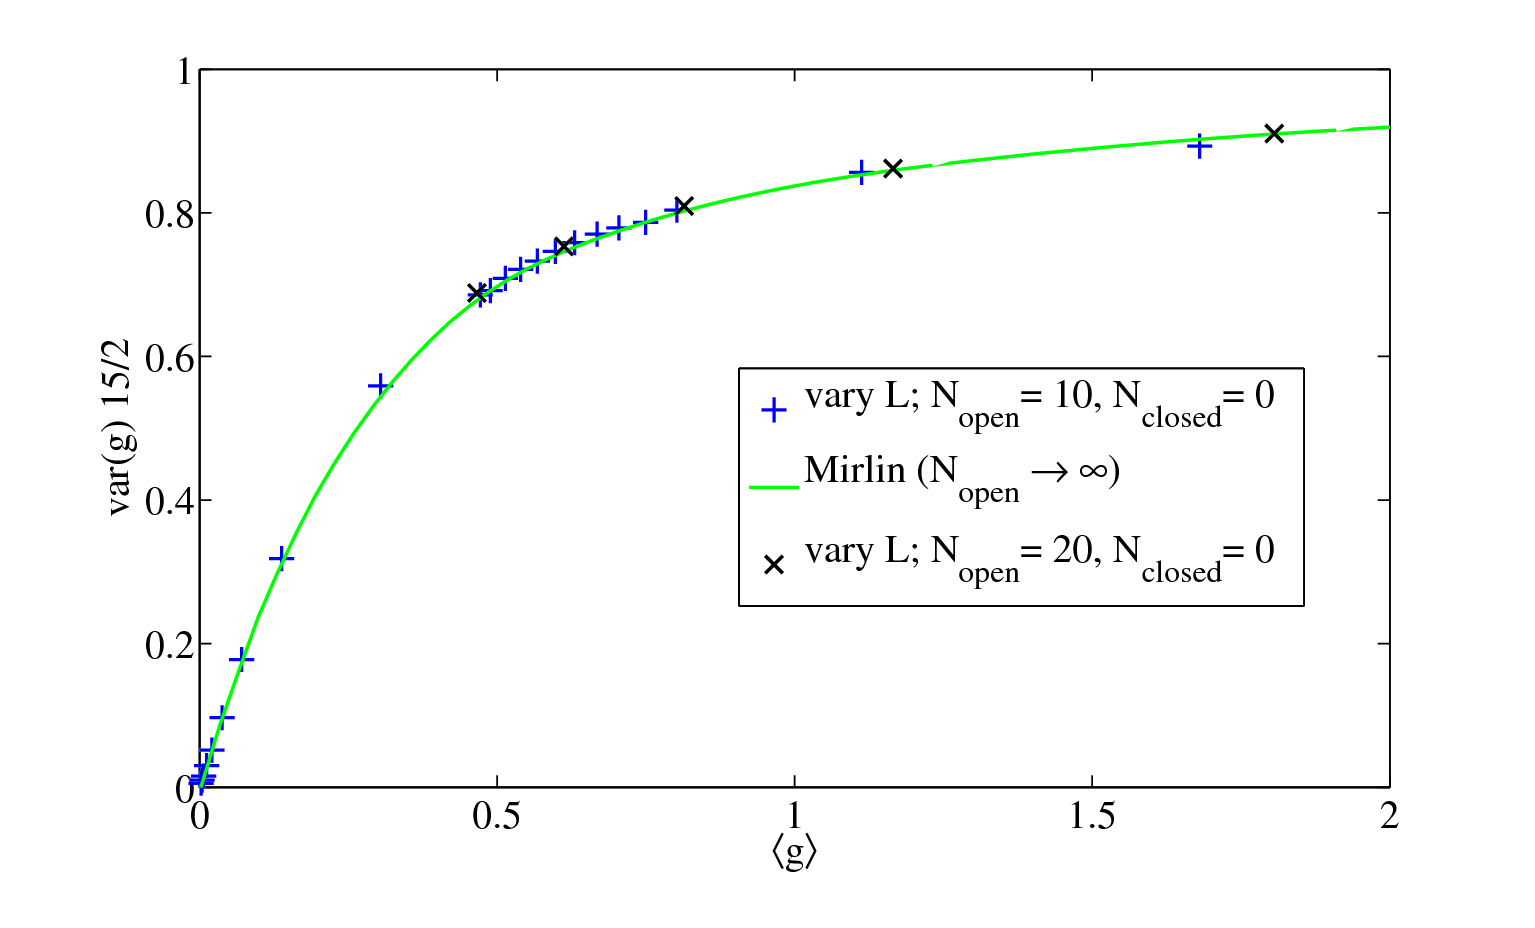
\includegraphics[width=3.25in]{pictures/var_g_versus_g_no_closed_channels}}}
\centerline{\rotatebox{0}{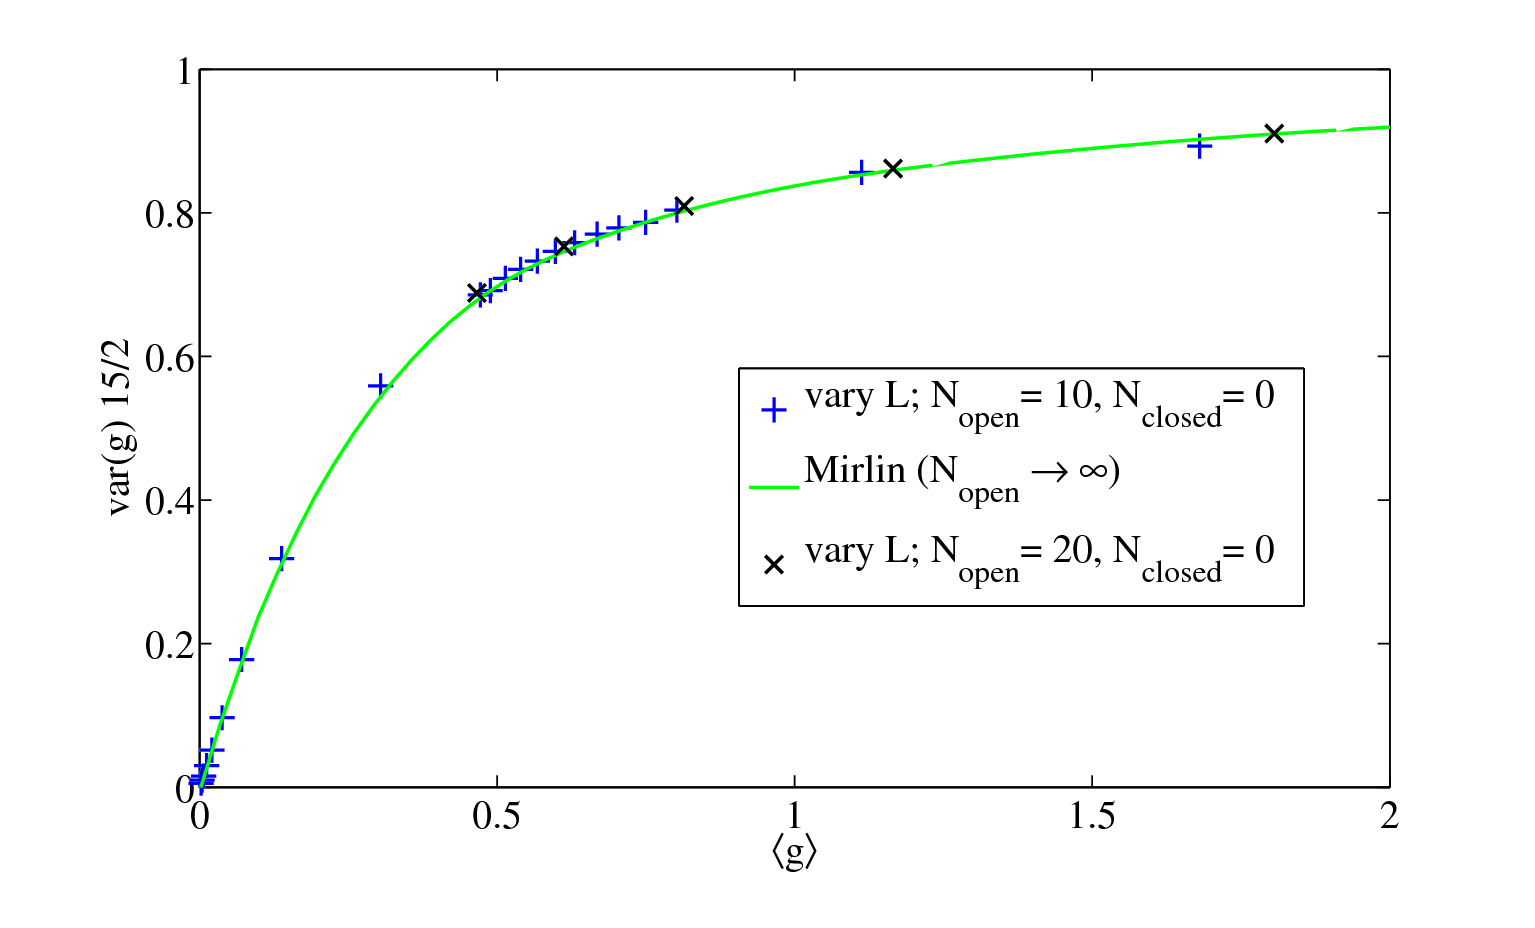
\includegraphics[width=3.25in]{pictures/var_g_versus_g_no_closed_channels}}}
%\begin{flushleft}
%(a)
%\end{flushleft}
%\vskip -0.7cm
%\centerline{\scalebox{0.35}{\includegraphics{pictures/periodic_34_defect_passive_to_gain2.eps}}}
%\begin{flushleft}
%(b)
%\end{flushleft}
%\vskip -0.7cm
%\centerline{\scalebox{0.35}{\includegraphics{pictures/periodic_14_defect_passive_to_gain2.eps}}}
%\vskip -0.0cm
\caption[Lorem ipsum dolor sit amet, consectetur adipiscing elit; Maecenas ultrices egestas commodo1D random medium.]{Lorem ipsum dolor sit amet, consectetur adipiscing elit; Maecenas ultrices egestas commodo1D random medium. Lorem ipsum dolor sit amet, consectetur adipiscing elit; Maecenas ultrices egestas commodo$x_0=L/4$ is considered. As discussed in Sec.~\ref{sec:correlation_te},Lorem ipsum dolor sit amet, consectetur adipiscing elit; Maecenas ultrices egestas commodo(such as those in Fig.~\ref{fig:Efield_random}) in random media. Panels (a) and (b) Lorem ipsum dolor sit amet, consectetur adipiscing elit; Maecenas ultrices egestas commodo(at resonant frequency) from the left and right respectively. Lorem ipsum dolor sit amet, consectetur adipiscing elit; Maecenas ultrices egestas commodo. The solid curves (from bottom up) are obtained for $l_{g,cr}/l_g$ equal to $0.5,\ 0.9,\ 0.99$ in (a) and $0.85,\ 0.95,\ 0.98,\ 0.99$ in (b). The field distribution in (b) Lorem ipsum dolor sit amet, consectetur adipiscing elit; Maecenas ultrices egestas commodo.\label{fig:localization_gain}}
\end{figure}
%%%%%%%%%%%%%%%%%%%%%%%%%%%%%%%%%%%%%%%%%%%%%%%%%%%%%%%%%%%%%%

As we observed in Sec.~\ref{sec:diffusion_general}, a change in $T/{\cal E}$Lorem ipsum dolor sit amet, consectetur adipiscing elit; Maecenas ultrices egestas commodo. Lorem ipsum dolor sit amet, consectetur adipiscing elit; Maecenas ultrices egestas commodo. Lorem ipsum dolor sit amet, consectetur adipiscing elit; Maecenas ultrices egestas commodo$\tilde{T}/\tilde{\cal E}$Lorem ipsum dolor sit amet, consectetur adipiscing elit; Maecenas ultrices egestas commodo. Interestingly,Lorem ipsum dolor sit amet, consectetur adipiscing elit; Maecenas ultrices egestas commodo. 

Lorem ipsum dolor sit amet, consectetur adipiscing elit; Maecenas ultrices egestas commodo, we employ the deterministic (non-random) Lorem ipsum dolor sit amet, consectetur adipiscing elit; Maecenas ultrices egestas commodo(see Sec.~\ref{sec:spectral_te}). Lorem ipsum dolor sit amet, consectetur adipiscing elit; Maecenas ultrices egestas commodo$\epsilon(x)\rightarrow\epsilon(x)+i\alpha$. As previously discussed in Sec.~\ref{sec:intro},Lorem ipsum dolor sit amet, consectetur adipiscing elit; Maecenas ultrices egestas commodo.

Lorem ipsum dolor sit amet, consectetur adipiscing elit; Maecenas ultrices egestas commodo.~\ref{fig:localization_gain}. Lorem ipsum dolor sit amet, consectetur adipiscing elit; Maecenas ultrices egestas commodo. Lorem ipsum dolor sit amet, consectetur adipiscing elit; Maecenas ultrices egestas commodo$x_T$,Lorem ipsum dolor sit amet, consectetur adipiscing elit; Maecenas ultrices egestas commodo, towards the sample boundary. Lorem ipsum dolor sit amet, consectetur adipiscing elit; Maecenas ultrices egestas commodo,Lorem ipsum dolor sit amet, consectetur adipiscing elit; Maecenas ultrices egestas commodo$E(x)$Lorem ipsum dolor sit amet, consectetur adipiscing elit; Maecenas ultrices egestas commodo. Lorem ipsum dolor sit amet, consectetur adipiscing elit; Maecenas ultrices egestas commodo.~\ref{sec:correlation_te}. 

At first glance,Lorem ipsum dolor sit amet, consectetur adipiscing elit; Maecenas ultrices egestas commodo.~\cite{2002_Jiang_Loc_Modes_Lasing,2002_Sebbah_Vanneste,2005_Vanneste} where (in localized regime) Lorem ipsum dolor sit amet, consectetur adipiscing elit; Maecenas ultrices egestas commodo. Lorem ipsum dolor sit amet, consectetur adipiscing elit; Maecenas ultrices egestas commodo. In our work,Lorem ipsum dolor sit amet, consectetur adipiscing elit; Maecenas ultrices egestas commodo, whereas in the previous works \cite{2002_Jiang_Loc_Modes_Lasing,2002_Sebbah_Vanneste,2005_Vanneste}Lorem ipsum dolor sit amet, consectetur adipiscing elit; Maecenas ultrices egestas commodo. Under such excitation conditions, the situation shown in Fig.~\ref{fig:localization_gain}a is always realized \cite{2010_Payne_loc_criterion}. Lorem ipsum dolor sit amet, consectetur adipiscing elit; Maecenas ultrices egestas commodo.~\ref{fig:localization_gain}Lorem ipsum dolor sit amet, consectetur adipiscing elit; Maecenas ultrices egestas commodo.~\ref{fig:localization_gain}Lorem ipsum dolor sit amet, consectetur adipiscing elit; Maecenas ultrices egestas commodo. Lorem ipsum dolor sit amet, consectetur adipiscing elit; Maecenas ultrices egestas commodo.

%%%%%%%%%%%%%%%%%%%%%%%%%%%%%%%%%%%%%%%%%%%%%%%%%%%%%%%%%
%\subsection{Gain-induced electric field modifications\label{sec:localization_gain_explained}} 
%%%%%%%%%%%%%%%%%%%%%%%%%%%%%%%%%%%%%%%%%%%%%%%%%%%%%%%%%

%%%%%%%%%%%%%%%%%%%%%%%%%%%%%%%%%%%%%%%%%%%%%%%%%%%%%%%%%%%%%%
\begin{figure*}
%\vskip -0.0cm
\centerline{\rotatebox{0}{
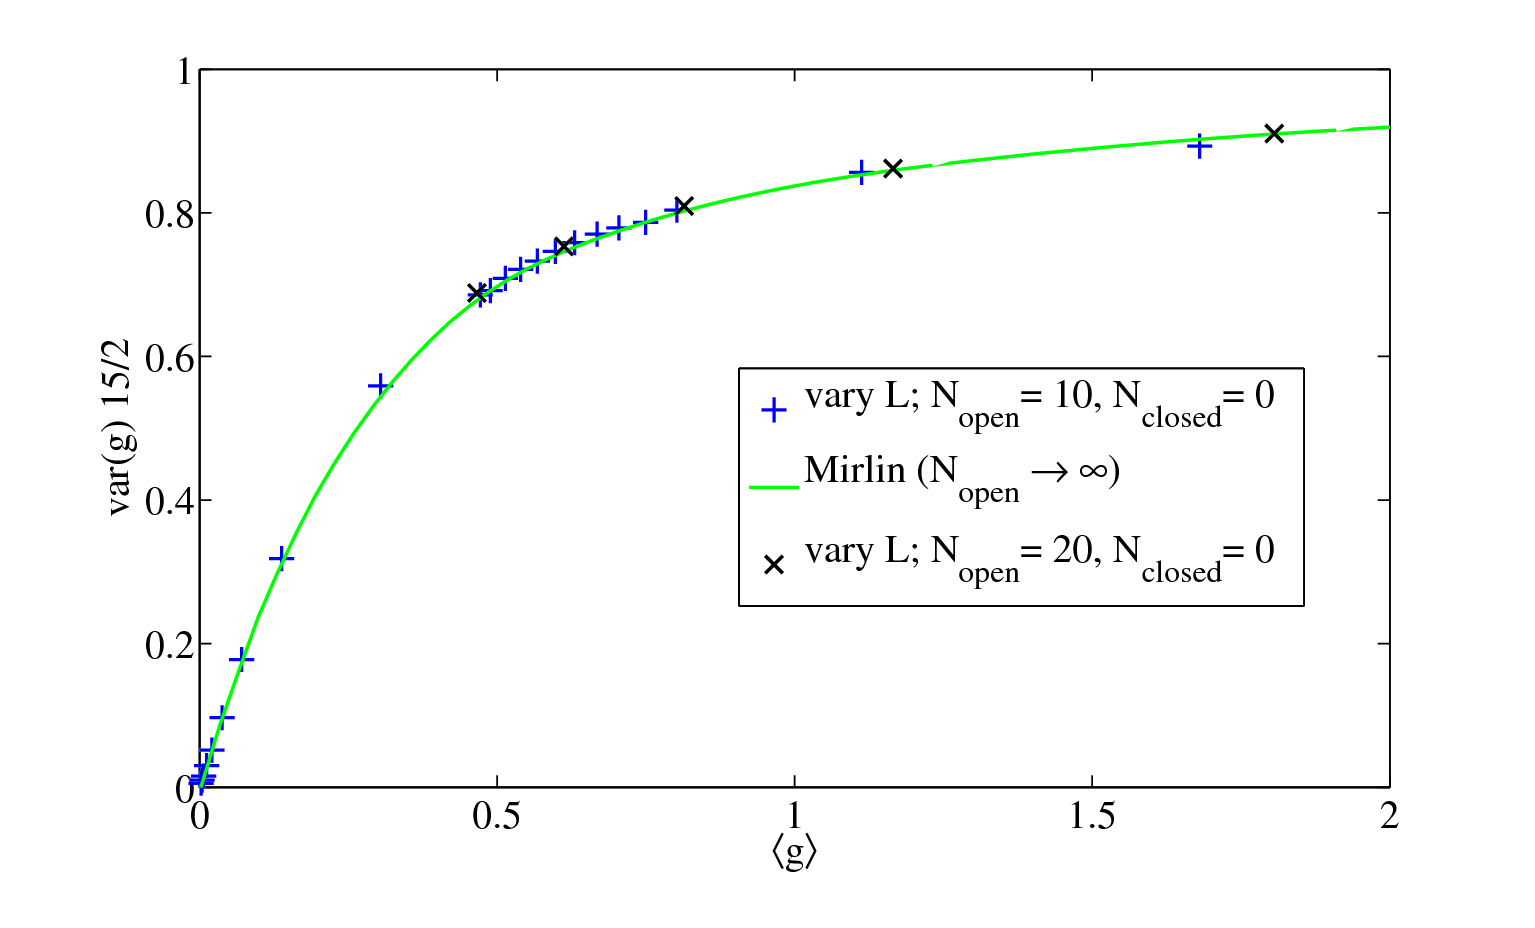
\includegraphics[width=2.25in]{pictures/var_g_versus_g_no_closed_channels}
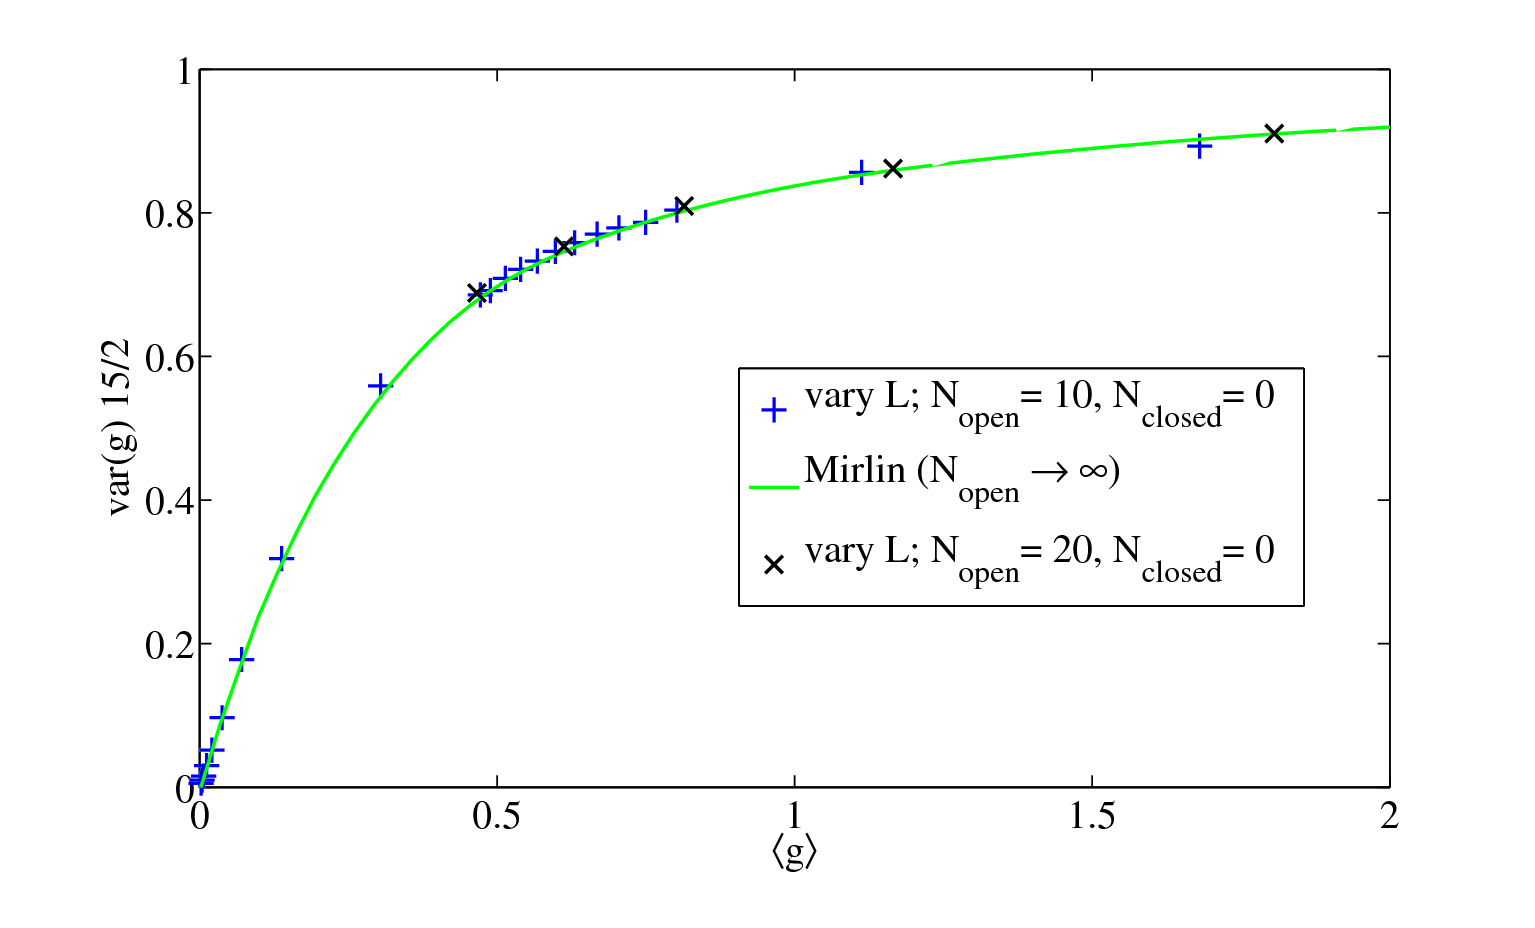
\includegraphics[width=2.25in]{pictures/var_g_versus_g_no_closed_channels}
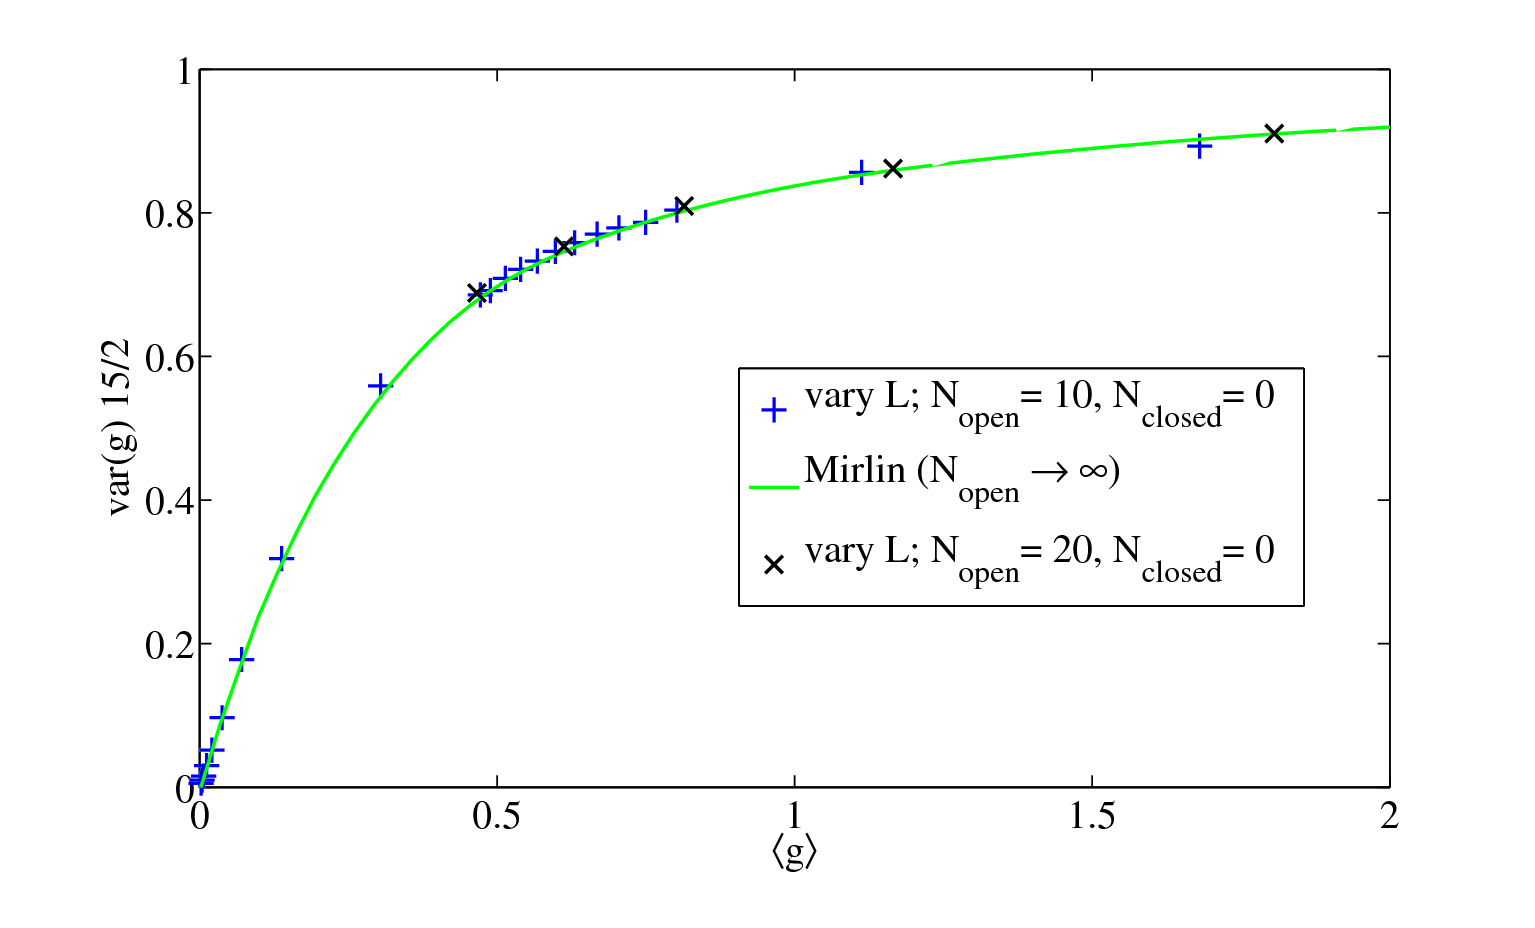
\includegraphics[width=2.25in]{pictures/var_g_versus_g_no_closed_channels}
}}
%\centerline{
%\scalebox{0.33}{\includegraphics{pictures/alpha_beta_electric_field}}
%\scalebox{0.33}{\includegraphics{pictures/alpha2_beta2}}
%\scalebox{0.33}{\includegraphics{pictures/alpha1_beta1}}}
%\vskip -0.0cm
\caption[Panel (a) plots $E_{L,R}(x,\omega_c)\equiv  E^{(L,R)}(x,\omega_c,\alpha=0)$Lorem ipsum dolor sit amet, consectetur adipiscing elit; Maecenas ultrices egestas commodo.]{Panel (a) plots $E_{L,R}(x,\omega_c)\equiv  E^{(L,R)}(x,\omega_c,\alpha=0)$Lorem ipsum dolor sit amet, consectetur adipiscing elit; Maecenas ultrices egestas commodo.~(\ref{eq:basis_functions_bc_l},\ref{eq:basis_functions_bc_r}), see text for notations. For non-zero gain, $\alpha>0$, the electric field distributions $E^{(L,R)}(x,\omega_c,\alpha)$Lorem ipsum dolor sit amet, consectetur adipiscing elit; Maecenas ultrices egestas commodo.~\ref{fig:localization_gain}. Lorem ipsum dolor sit amet, consectetur adipiscing elit; Maecenas ultrices egestas commodo(a), and the resulting coefficients $C_{L,R}^{(L)}(\alpha)$ and $C_{L,R}^{(R)}(\alpha)$, defined in Eq.~(\ref{eq:C_completeness}), are plotted in (b) and (c) respectively. Lorem ipsum dolor sit amet, consectetur adipiscing elit; Maecenas ultrices egestas commodo$E_{L}(x,\omega_c)$ and $E^{(c)}(x,\omega_c)$ (the solution in the closed system) Lorem ipsum dolor sit amet, consectetur adipiscing elit; Maecenas ultrices egestas commodo,Lorem ipsum dolor sit amet, consectetur adipiscing elit; Maecenas ultrices egestas commodo. In all three panels, thick / thin curve and large / small symbols refer to  $E_{L}(x,\omega_c)$ / $E_{R}(x,\omega_c)$.\label{fig:alphabeta}}
\end{figure*}
%%%%%%%%%%%%%%%%%%%%%%%%%%%%%%%%%%%%%%%%%%%%%%%%%%%%%%%%%%%%%%

Lorem ipsum dolor sit amet, consectetur adipiscing elit; Maecenas ultrices egestas commodo. 

Lorem ipsum dolor sit amet, consectetur adipiscing elit; Maecenas ultrices egestas commodo. Lorem ipsum dolor sit amet, consectetur adipiscing elit; Maecenas ultrices egestas commodo(reflected and transmitted) signals. Lorem ipsum dolor sit amet, consectetur adipiscing elit; Maecenas ultrices egestas commodo(CW) Lorem ipsum dolor sit amet, consectetur adipiscing elit; Maecenas ultrices egestas commodo. Lorem ipsum dolor sit amet, consectetur adipiscing elit; Maecenas ultrices egestas commodo(linearly independent) solution for the same frequency. In general, any two (because Maxwell'Lorem ipsum dolor sit amet, consectetur adipiscing elit; Maecenas ultrices egestas commodo) Lorem ipsum dolor sit amet, consectetur adipiscing elit; Maecenas ultrices egestas commodo$\omega$. 

Lorem ipsum dolor sit amet, consectetur adipiscing elit; Maecenas ultrices egestas commodo1Lorem ipsum dolor sit amet, consectetur adipiscing elit; Maecenas ultrices egestas commodo.~(\ref{eq:basis_functions_bc_l},\ref{eq:basis_functions_bc_r}). They correspond to the left- and right-Lorem ipsum dolor sit amet, consectetur adipiscing elit; Maecenas ultrices egestas commodo.~\ref{sec:correlation_te} and Appx.~\ref{app:qm_model} with $r_{L,R}(\omega),t_{L,R}(\omega)$Lorem ipsum dolor sit amet, consectetur adipiscing elit; Maecenas ultrices egestas commodo. Lorem ipsum dolor sit amet, consectetur adipiscing elit; Maecenas ultrices egestas commodo(it is independent of $x$ in our model of disorder $\epsilon(x)$) is non-zero for one particular value of $x$. At $x=0$Lorem ipsum dolor sit amet, consectetur adipiscing elit; Maecenas ultrices egestas commodo.~(\ref{eq:basis_functions_bc_l},\ref{eq:basis_functions_bc_r}) as $-2it_R(\omega)\omega/c\neq 0$.

At some special frequencies $\omega_c$, a linear combination  $E^{(c)}(x,\omega_c)=C_L^{(c)} E_{L}(x,\omega_c)+C_R^{(c)} E_{R}(x,\omega_c)$ can be formed such that conditions $E^{(c)}(x=0,\omega_c)=0$ and $E^{(c)}(x=L,\omega_c)=0$ are satisfied simultaneously. Such $\omega_c$'s  correspond to the true eigen-modes of the closed system -- the system defined by $\epsilon(0\leq x\leq L)$ with zero (reflecting) boundary conditions at $x=0,L$. Lorem ipsum dolor sit amet, consectetur adipiscing elit; Maecenas ultrices egestas commodo1Lorem ipsum dolor sit amet, consectetur adipiscing elit; Maecenas ultrices egestas commodo(similar to $E_{L}(x,\omega_c)$ depicted with thick lines in Figs. (\ref{fig:Efield_random},\ref{fig:barrierdefectlog})) makes the dominant contribution to $E^{(c)}(x,\omega_c)$. Lorem ipsum dolor sit amet, consectetur adipiscing elit; Maecenas ultrices egestas commodo(similar to $E_{R}(x,\omega_c)$ depicted with thin lines in Figs. (\ref{fig:Efield_random},\ref{fig:barrierdefectlog})) Lorem ipsum dolor sit amet, consectetur adipiscing elit; Maecenas ultrices egestas commodo.~\cite{2002_Jiang_Loc_Modes_Lasing,2002_Sebbah_Vanneste,2005_Vanneste}.

Lorem ipsum dolor sit amet, consectetur adipiscing elit; Maecenas ultrices egestas commodo, $\alpha>0$,Lorem ipsum dolor sit amet, consectetur adipiscing elit; Maecenas ultrices egestas commodo, $E^{(L)}(x,\omega_c,\alpha)$, and from the right $E^{(R)}(x,\omega_c,\alpha)$, c.f.~Fig.~\ref{fig:localization_gain}. In this case, the distributions can no longer, strictly speaking, be expressed in terms of $E_{L,R}(x,\omega_c)\equiv  E^{(L,R)}(x,\omega_c,\alpha=0)$. However,Lorem ipsum dolor sit amet, consectetur adipiscing elit; Maecenas ultrices egestas commodo, $\alpha<\alpha_{cr}\ll\omega_c$,Lorem ipsum dolor sit amet, consectetur adipiscing elit; Maecenas ultrices egestas commodo$E_{L,R}(x,\omega_c)$Lorem ipsum dolor sit amet, consectetur adipiscing elit; Maecenas ultrices egestas commodo$E(x,\omega_c,\alpha)$Lorem ipsum dolor sit amet, consectetur adipiscing elit; Maecenas ultrices egestas commodo$\alpha$-dependent $C_{L}(\alpha)$,$C_{R}(\alpha)$:
\begin{equation}
E(x,\omega_c,\alpha)\simeq C_L(\alpha) E_{L}(x,\omega_c)+C_R(\alpha) E_{R}(x,\omega_c).
\label{eq:C_decomposition}
\end{equation}
Lorem ipsum dolor sit amet, consectetur adipiscing elit; Maecenas ultrices egestas commodo.~(\ref{eq:C_decomposition}) is verified numerically by computing  
\begin{equation}
C_{L,R}^{(L,R)}(\alpha)=\int_{0}^{L} E^{(L,R)}(x,\omega_c,\alpha)E_{L,R}^*(x,\omega_c)dx.
\label{eq:C_completeness}
\end{equation}
Figs.~\ref{fig:alphabeta}b,c show $C_{L,R}^{(L)}(\alpha)$ and $C_{L,R}^{(R)}(\alpha)$ respectively. Lorem ipsum dolor sit amet, consectetur adipiscing elit; Maecenas ultrices egestas commodo$x_0\sim L/4$ where passive profiles, depicted in Fig.~\ref{fig:alphabeta}a,Lorem ipsum dolor sit amet, consectetur adipiscing elit; Maecenas ultrices egestas commodo.~\ref{fig:Efield_random},\ref{fig:barrierdefectlog},\ref{fig:localization_gain}. When gain is added to the system, we observe that $E^{(L)}(x,\omega_c,\alpha)\propto E_{L}(x,\omega_c)$ for all values of gain, c.f.~Fig.~\ref{fig:alphabeta}b. In contrast, $E^{(R)}(x,\omega_c,\alpha)$ exhibited a crossover behavior from $E^{(R)}(x,\omega_c,\alpha)\propto E_{R}(x,\omega_c)$ for small $\alpha$, to $E^{(R)}(x,\omega_c,\alpha)\propto E_{L}(x,\omega_c)$ in the vicinity of lasing threshold. Lorem ipsum dolor sit amet, consectetur adipiscing elit; Maecenas ultrices egestas commodo.~\ref{sec:localization_gain}, c.f.~Fig.~\ref{fig:localization_gain},Lorem ipsum dolor sit amet, consectetur adipiscing elit; Maecenas ultrices egestas commodo. Lorem ipsum dolor sit amet, consectetur adipiscing elit; Maecenas ultrices egestas commodo(at the same frequency),Lorem ipsum dolor sit amet, consectetur adipiscing elit; Maecenas ultrices egestas commodo-boundaries. Lorem ipsum dolor sit amet, consectetur adipiscing elit; Maecenas ultrices egestas commodo. 

Finally, we note that the solutions $E_{L,R}(x,\omega)$ should not be confused with the quasi-mode $E(x,\omega_c+i\varepsilon)$Lorem ipsum dolor sit amet, consectetur adipiscing elit; Maecenas ultrices egestas commodo$\omega_c+i\varepsilon$ where e.g. transmission becomes singular. Such quasi-Lorem ipsum dolor sit amet, consectetur adipiscing elit; Maecenas ultrices egestas commodo. However, for a uniform gain in the form $\epsilon(x)(1+i\alpha)$ the dominant mode profile $E^{(L)}(x,\omega_c,\alpha_{cr})$ does indeed coincide with the quasi-mode due to equivalence between $\epsilon(x)(1+i\alpha)\omega_c/c$ and $\epsilon(x)(\omega_c+i\varepsilon)/c$.

%%%%%%%%%%%%%%%%%%%%%%%%%%%%%%%%%%%%%%%%%%%%%%%%%%%%%%%%%
\section{DISCUSSION AND OUTLOOK}
\label{sec:discussion_TE}
%%%%%%%%%%%%%%%%%%%%%%%%%%%%%%%%%%%%%%%%%%%%%%%%%%%%%%%%%

Lorem ipsum dolor sit amet, consectetur adipiscing elit; Maecenas ultrices egestas commodo. Lorem ipsum dolor sit amet, consectetur adipiscing elit; Maecenas ultrices egestas commodo, thus,Lorem ipsum dolor sit amet, consectetur adipiscing elit; Maecenas ultrices egestas commodo\cite{2004_Yamilov_intensity,2005_Yamilov_correlations,2006_Yamilov_conductance}. 

In Sec.~\ref{sec:diffusion_section}Lorem ipsum dolor sit amet, consectetur adipiscing elit; Maecenas ultrices egestas commodo-averaged quantities $T/{\cal E}$Lorem ipsum dolor sit amet, consectetur adipiscing elit; Maecenas ultrices egestas commodo, Eq.~(\ref{eq:TE_vs_D}), in a passive random medium. Lorem ipsum dolor sit amet, consectetur adipiscing elit; Maecenas ultrices egestas commodo(decrease) of the $T/{\cal E}$Lorem ipsum dolor sit amet, consectetur adipiscing elit; Maecenas ultrices egestas commodo-renormalized diffusion coefficient $D(z)\equiv D_0=c\ell/3$Lorem ipsum dolor sit amet, consectetur adipiscing elit; Maecenas ultrices egestas commodo. 

In Sec.~\ref{sec:diffusion_general} we obtained the expressions for $T$ and ${\cal E}$Lorem ipsum dolor sit amet, consectetur adipiscing elit; Maecenas ultrices egestas commodo. Lorem ipsum dolor sit amet, consectetur adipiscing elit; Maecenas ultrices egestas commodo, we conjecture that the decrease in $T/{\cal E}$ below the level established by Eq.~(\ref{eq:TE_analytical}) Lorem ipsum dolor sit amet, consectetur adipiscing elit; Maecenas ultrices egestas commodo. Lorem ipsum dolor sit amet, consectetur adipiscing elit; Maecenas ultrices egestas commodo.

Lorem ipsum dolor sit amet, consectetur adipiscing elit; Maecenas ultrices egestas commodo-to-sample fluctuations,Lorem ipsum dolor sit amet, consectetur adipiscing elit; Maecenas ultrices egestas commodo, the ratio between $\tilde{T}$ and $\tilde{\cal E}$Lorem ipsum dolor sit amet, consectetur adipiscing elit; Maecenas ultrices egestas commodo. Lorem ipsum dolor sit amet, consectetur adipiscing elit; Maecenas ultrices egestas commodo, c.f.~Sec.~\ref{sec:localization_passive}. Although the ratio $\tilde{T}/\tilde{\cal E}$Lorem ipsum dolor sit amet, consectetur adipiscing elit; Maecenas ultrices egestas commodo,Lorem ipsum dolor sit amet, consectetur adipiscing elit; Maecenas ultrices egestas commodo(or, equivalently, the direction of the incident wave) even in the passive system, c.f.~Sec.~\ref{sec:correlation_te}. In Sec.~\ref{sec:spectral_te},\ref{app:qm_model}Lorem ipsum dolor sit amet, consectetur adipiscing elit; Maecenas ultrices egestas commodo. This is unlike the transmission $\tilde{T}$,Lorem ipsum dolor sit amet, consectetur adipiscing elit; Maecenas ultrices egestas commodo(because of reciprocity) --Lorem ipsum dolor sit amet, consectetur adipiscing elit; Maecenas ultrices egestas commodo.~\ref{fig:Efield_random}. Lorem ipsum dolor sit amet, consectetur adipiscing elit; Maecenas ultrices egestas commodo,Lorem ipsum dolor sit amet, consectetur adipiscing elit; Maecenas ultrices egestas commodo,Lorem ipsum dolor sit amet, consectetur adipiscing elit; Maecenas ultrices egestas commodo: $\tilde{T}_G(\alpha)=\left(\tilde{T}(\alpha)/\tilde{\cal E}(\alpha)\right)\times\tilde{\cal E}_0$. Here $\tilde{\cal E}_0\equiv\tilde{\cal E}(\alpha=0)$Lorem ipsum dolor sit amet, consectetur adipiscing elit; Maecenas ultrices egestas commodo. Lorem ipsum dolor sit amet, consectetur adipiscing elit; Maecenas ultrices egestas commodo$\tilde{T}_G$Lorem ipsum dolor sit amet, consectetur adipiscing elit; Maecenas ultrices egestas commodo. By construction, $\tilde{T}_G(\alpha)$ reduces to the transmission in a 1D system without gain ($\alpha\rightarrow 0$) Lorem ipsum dolor sit amet, consectetur adipiscing elit; Maecenas ultrices egestas commodo(average) Lorem ipsum dolor sit amet, consectetur adipiscing elit; Maecenas ultrices egestas commodo. Hence, one can refer to $T_G$ as generalized transmission (conductance).

In future,Lorem ipsum dolor sit amet, consectetur adipiscing elit; Maecenas ultrices egestas commodo$\tilde{T}(\alpha)/\tilde{{\cal E}}(\alpha)$ and $T_G(\alpha)$ in random medium with gain. Experimentally,Lorem ipsum dolor sit amet, consectetur adipiscing elit; Maecenas ultrices egestas commodo-field scanning measurements in two-dimensional random media --Lorem ipsum dolor sit amet, consectetur adipiscing elit; Maecenas ultrices egestas commodo. Lorem ipsum dolor sit amet, consectetur adipiscing elit; Maecenas ultrices egestas commodo. 

%%%%%%%%%%%%%%%%%%%%%%%%%%%%%%%%%%%%%%%%%%%%%%%%%%%%%%%%%
\section{ACKNOWLEDGMENTS}
%%%%%%%%%%%%%%%%%%%%%%%%%%%%%%%%%%%%%%%%%%%%%%%%%%%%%%%%%
 
Lorem ipsum dolor sit amet, consectetur adipiscing elit; Maecenas ultrices egestas commodo. DMR-0704981 and DMR-0808937. The numerical
results obtained at the Tera-Grid, Grants No. DMR-090132 and No. DMR-100030. AY is grateful to S. Skipetrov, A. Lagendijk and B. van Tiggelen for valuable comments.

\section{APPENDIX}
%\appendix

\subsection{Derivation of Equation~(\ref{eq:TE_vs_D})}
\label{app:Dz_derivation}
We consider a slab geometry,Lorem ipsum dolor sit amet, consectetur adipiscing elit; Maecenas ultrices egestas commodo$z$Lorem ipsum dolor sit amet, consectetur adipiscing elit; Maecenas ultrices egestas commodo${\bf \rho}$ as ${\bf r}=({\bf \rho},z)$. Assuming no dependence on ${\bf \rho}$ allows us to rewrite Eq.~(\ref{eq:Jflux}) in the form
\begin{equation}
\langle J_z(z)\rangle=
\displaystyle -D(z)\frac{d\langle {\cal W}(z)\rangle}{dz}.
\label{eq:Jfluxz}
\end{equation}
Independence of ${\bf \rho}$ is insured for the plane-Lorem ipsum dolor sit amet, consectetur adipiscing elit; Maecenas ultrices egestas commodo. 

Lorem ipsum dolor sit amet, consectetur adipiscing elit; Maecenas ultrices egestas commodo${\cal W}(z)$ is stationary, $\partial \langle {\cal W}(z)\rangle/\partial t=0$, it follows from Eq.~(\ref{eq:Jflux_conserv}) that the $z$-component of flux is constant for $z>z_p\sim\ell$. Lorem ipsum dolor sit amet, consectetur adipiscing elit; Maecenas ultrices egestas commodo$z=L$ as
\begin{equation}
\langle J_z(z)\rangle=\left\{
\begin{array}{l l}
\langle J_z(L)\rangle\equiv J_0 T,&\quad z_p<z<L\\
\langle J_z(0)\rangle\equiv -J_0 R,&\quad 0<z<z_p\\
\end{array} \right.
\label{eq:Jfluxz_const}
\end{equation}
where $T$ is the transmission coefficient. Furthermore, by integrating Eq.~(\ref{eq:Jflux_conserv}) Lorem ipsum dolor sit amet, consectetur adipiscing elit; Maecenas ultrices egestas commodo$\langle J_z(L)\rangle -\langle J_z(0)\rangle =J_0 T-(-J_0 R)=J_0(T+R)=J_0$.

After establishing Eq.~(\ref{eq:Jfluxz_const}),Lorem ipsum dolor sit amet, consectetur adipiscing elit; Maecenas ultrices egestas commodo.~(\ref{eq:Jfluxz}). An integration over $z$ gives
\begin{equation}
\displaystyle\int_z^L\frac{\langle J_z(z^\prime)\rangle dz^\prime}{D(z^\prime)}=-\langle {\cal W}(L)\rangle + \langle {\cal W}(z)\rangle.
\label{eq:E1}
\end{equation}
The energy density $\langle {\cal W}(L)\rangle$Lorem ipsum dolor sit amet, consectetur adipiscing elit; Maecenas ultrices egestas commodo- and left-propagating fluxes $\langle J_+(L)\rangle=J_0T$, $\langle J_-(L)\rangle=0$ using Eqs.~(\ref{eq:diffusive_flux}). We obtain $\langle {\cal W}(L)\rangle=2J_0T/c$. To take advantage of the fact that $\langle J_z(z)\rangle$ is piecewise constant, c.f.~Eq.~(\ref{eq:Jfluxz_const}), we have to neglect by $0<z<z_p$ contribution. This introduces an error $\propto z_p/L\sim\ell/L\ll 1$,Lorem ipsum dolor sit amet, consectetur adipiscing elit; Maecenas ultrices egestas commodo$T$ and $D(z)$ contributions as
\begin{equation}
J_0T\left[\displaystyle\int_z^L\frac{dz^\prime}{D(z^\prime)}+2/c\right]= \langle {\cal W}(z)\rangle.
\label{eq:E1a}
\end{equation}
Before proceeding further,Lorem ipsum dolor sit amet, consectetur adipiscing elit; Maecenas ultrices egestas commodo$\sim \ell/L$Lorem ipsum dolor sit amet, consectetur adipiscing elit; Maecenas ultrices egestas commodo. Hence, $2/c$ contribution has to be dropped as well.

A subsequent integration of Eq.~(\ref{eq:E1a}) gives 
\begin{equation}
J_0T\displaystyle\int_{0}^{L}\int_{z}^{L}\displaystyle\frac{1}{D(z^\prime)}dz^\prime dz=
\displaystyle\int_0^L \langle {\cal W}(z)\rangle dz
\equiv{\cal E}
\label{eq:E2}
\end{equation}
Taking advantage of the system symmetry, $D(z)=D(L-z)$,Lorem ipsum dolor sit amet, consectetur adipiscing elit; Maecenas ultrices egestas commodo
\begin{eqnarray}
\displaystyle\int_{0}^{L}\int_{z}^{L}\displaystyle\frac{1}{D(z^\prime)}dz^\prime dz &=&\frac{1}{2}\displaystyle\int_{0}^{L}\int_{0}^{L}\displaystyle\frac{1}{D(z^\prime)}dz^\prime dz \nonumber\\
&=&\frac{L}{2}\int_{0}^{L}\displaystyle\frac{1}{D(z)}dz.
\label{eq:E3}
\end{eqnarray}
Lorem ipsum dolor sit amet, consectetur adipiscing elit; Maecenas ultrices egestas commodo, $D(z)=D_0\equiv c\ell/3$, we obtain Eq.~(\ref{eq:TE_vs_D}).

\subsection{Dependence of \texorpdfstring{$\tilde{T}/\tilde{\cal E}$}{T/E} on Position of the Defect State: Non-random Model}
\label{app:qm_model}
%%%%%%%%%%%%%%%%%%%%%%%%%%%%%%%%%%%%%%%%%%%%%%%%%%%%%%%%%

Lorem ipsum dolor sit amet, consectetur adipiscing elit; Maecenas ultrices egestas commodo-dependent energy content as in Fig.~\ref{fig:Efield_random}Lorem ipsum dolor sit amet, consectetur adipiscing elit; Maecenas ultrices egestas commodo. 

A clarification is in order. There is no one-to-Lorem ipsum dolor sit amet, consectetur adipiscing elit; Maecenas ultrices egestas commodo\"{o}dinger and Helmholtz equations\cite{2004_dragoman_book}. Indeed, John \cite{1991_John}Lorem ipsum dolor sit amet, consectetur adipiscing elit; Maecenas ultrices egestas commodo, strictly speaking, applied to the electromagnetic waves. However,Lorem ipsum dolor sit amet, consectetur adipiscing elit; Maecenas ultrices egestas commodo\cite{1987_John} (e.g. disordered photonic crystals), the negative energy and, thus, tunneling regime can be recovered. To achieve this formally,Lorem ipsum dolor sit amet, consectetur adipiscing elit; Maecenas ultrices egestas commodo-medium transformation, as in e.g. Refs \cite{1994_Sipe,2004_Bliokh_wavelet,2008_Yamilov_JoSAB}. 

Lorem ipsum dolor sit amet, consectetur adipiscing elit; Maecenas ultrices egestas commodo. In particular,Lorem ipsum dolor sit amet, consectetur adipiscing elit; Maecenas ultrices egestas commodo(at $x_0=L/4$) and the second (at $x_0=3L/4$) half of of the system. Lorem ipsum dolor sit amet, consectetur adipiscing elit; Maecenas ultrices egestas commodo.~\ref{fig:barrierdefectlog}. As in Sec.~\ref{sec:correlation_te}, $x_0=3L/4$Lorem ipsum dolor sit amet, consectetur adipiscing elit; Maecenas ultrices egestas commodo.

Lorem ipsum dolor sit amet, consectetur adipiscing elit; Maecenas ultrices egestas commodo\"{o}Lorem ipsum dolor sit amet, consectetur adipiscing elit; Maecenas ultrices egestas commodo(Lorem ipsum dolor sit amet, consectetur adipiscing elit; Maecenas ultrices egestas commodo) Lorem ipsum dolor sit amet, consectetur adipiscing elit; Maecenas ultrices egestas commodo. Fig.~\ref{fig:barrierdefectlog}Lorem ipsum dolor sit amet, consectetur adipiscing elit; Maecenas ultrices egestas commodo. Lorem ipsum dolor sit amet, consectetur adipiscing elit; Maecenas ultrices egestas commodo,Lorem ipsum dolor sit amet, consectetur adipiscing elit; Maecenas ultrices egestas commodo$L/4$ and $3L/4$,Lorem ipsum dolor sit amet, consectetur adipiscing elit; Maecenas ultrices egestas commodo. Lorem ipsum dolor sit amet, consectetur adipiscing elit; Maecenas ultrices egestas commodo-on-Lorem ipsum dolor sit amet, consectetur adipiscing elit; Maecenas ultrices egestas commodo\ref{sec:numerical_model},\ref{sec:correlation_te}. In the case of $x_0=3L/4$ defect,Lorem ipsum dolor sit amet, consectetur adipiscing elit; Maecenas ultrices egestas commodo$x_T$, where $x_T$ is the turning point. The position of $x_T$Lorem ipsum dolor sit amet, consectetur adipiscing elit; Maecenas ultrices egestas commodo.~\ref{fig:barrierdefectlog},Lorem ipsum dolor sit amet, consectetur adipiscing elit; Maecenas ultrices egestas commodo.

%%%%%%%%%%%%%%%%%%%%%%%%%%%%%%%%%%%%%%%
\begin{figure}%[t]
\centerline{\rotatebox{0}{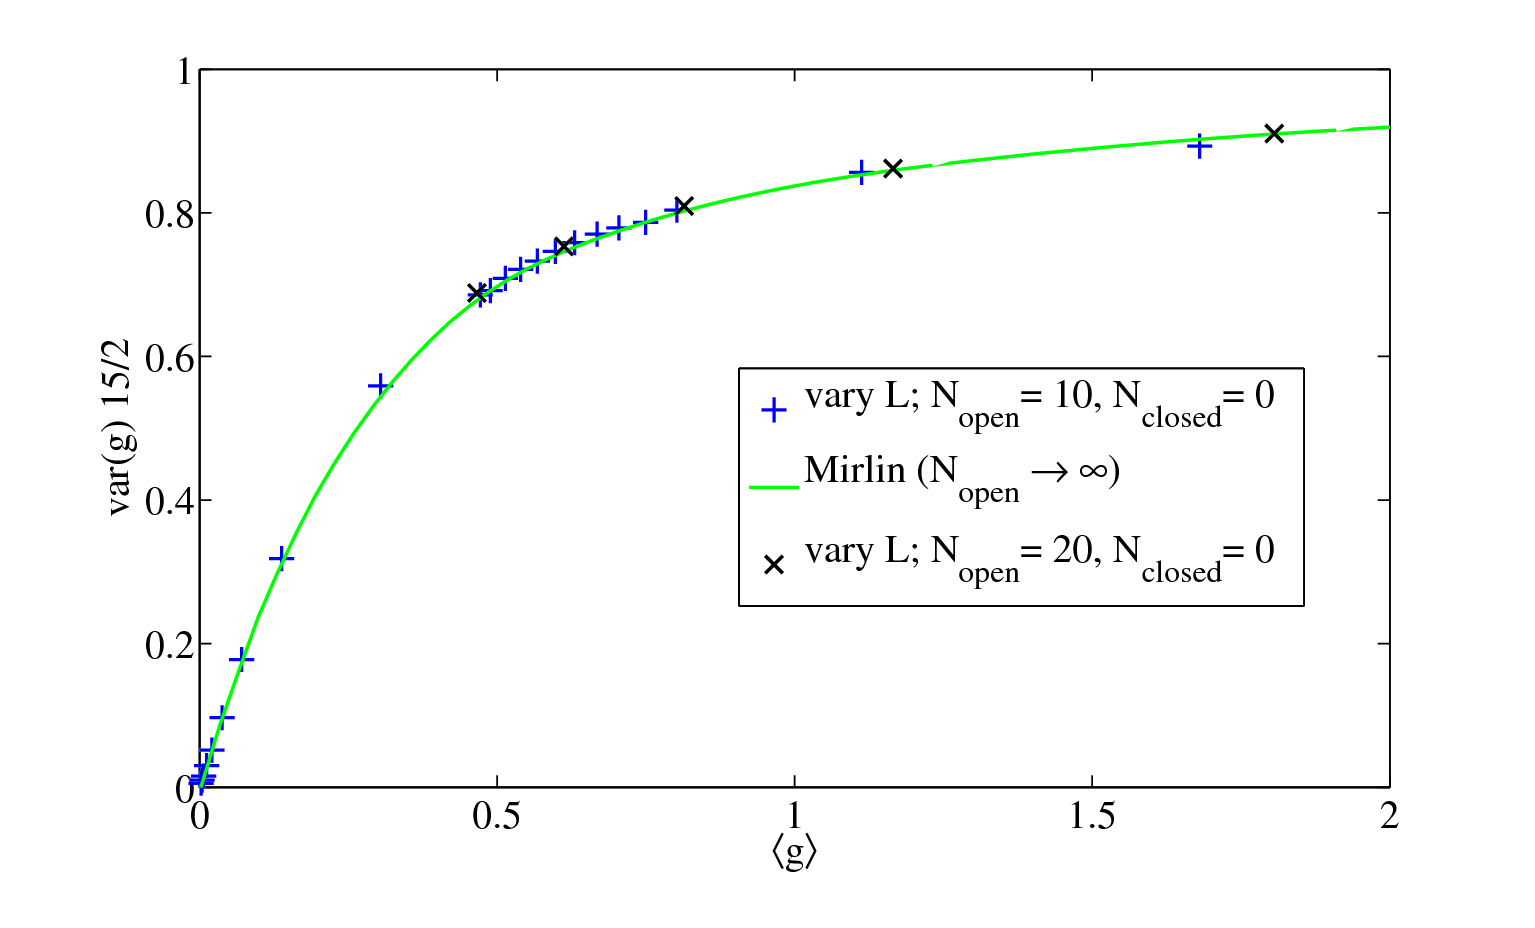
\includegraphics[width=3.25in]{pictures/var_g_versus_g_no_closed_channels}}}
%\vskip -0.0in
%\scalebox{0.37}{\includegraphics{pictures/barrier_defect_at_14_and_34_waveform_log_chopped.eps}}
%\vskip -0.2in
\caption[Solution of the Schr\"{o}Lorem ipsum dolor sit amet, consectetur adipiscing elit; Maecenas ultrices egestas commodo.]{Solution of the Schr\"{o}Lorem ipsum dolor sit amet, consectetur adipiscing elit; Maecenas ultrices egestas commodo. Lorem ipsum dolor sit amet, consectetur adipiscing elit; Maecenas ultrices egestas commodo-Lorem ipsum dolor sit amet, consectetur adipiscing elit; Maecenas ultrices egestas commodo. Lorem ipsum dolor sit amet, consectetur adipiscing elit; Maecenas ultrices egestas commodo(thick line) and the right (thin line) Lorem ipsum dolor sit amet, consectetur adipiscing elit; Maecenas ultrices egestas commodo.~\ref{fig:Efield_random}.\label{fig:barrierdefectlog}}
\end{figure}
%%%%%%%%%%%%%%%%%%%%%%%%%%%%%%%%%%%%%%%


\begin{table}
\begin{center}
\caption{\label{tab:asdf}Nearest and next-nearest pairings kazoo}
\begin{tabular}{||c|c|c||c|c|c||}
\hline
$c^{(nn)}_{1}$ & $c^{(nn)}_{2}$ & $c^{(nn)}_{3}$ & $c^{(nnn)}_{1}$ & $c^{(nnn)}_{2}$ & $c^{(nnn)}_{3}$ \\ \hline
$0.004105$ & $0.000915$ & $0.000238$ & $0.002034$ & $0.000736$ & $0.000261$ \\
% from /svn/research/Project_DAS/2012_TB_for_2DTM_manuscript/TB_for_2DTM.xlsx SVN 3082
\hline
\end{tabular}
\end{center}
\end{table}


The non-Lorem ipsum dolor sit amet, consectetur adipiscing elit; Maecenas ultrices egestas commodo. Lorem ipsum dolor sit amet, consectetur adipiscing elit; Maecenas ultrices egestas commodo-Lorem ipsum dolor sit amet, consectetur adipiscing elit; Maecenas ultrices egestas commodo(in the electromagnetic problem,Lorem ipsum dolor sit amet, consectetur adipiscing elit; Maecenas ultrices egestas commodo). Lorem ipsum dolor sit amet, consectetur adipiscing elit; Maecenas ultrices egestas commodo. It appears that in the $x_0=3L/4$ case,Lorem ipsum dolor sit amet, consectetur adipiscing elit; Maecenas ultrices egestas commodo,Lorem ipsum dolor sit amet, consectetur adipiscing elit; Maecenas ultrices egestas commodo$x_T$. In contrast,Lorem ipsum dolor sit amet, consectetur adipiscing elit; Maecenas ultrices egestas commodo,Lorem ipsum dolor sit amet, consectetur adipiscing elit; Maecenas ultrices egestas commodo.

Lorem ipsum dolor sit amet, consectetur adipiscing elit; Maecenas ultrices egestas commodo.~\ref{sec:localization_passive}.

